\documentclass[english,12pt]{article}


\usepackage{amsmath}
\usepackage{balance}  % to better equalize the last page
%%\usepackage{graphics} % for EPS, load graphicx instead
\usepackage{graphicx}
% \usepackage{subfigure}
\usepackage[font = small]{caption}
\usepackage{subcaption}
\usepackage{txfonts}
\usepackage{color}
\usepackage{cite}
\usepackage{textcomp}
\usepackage{geometry}
\usepackage{booktabs}
\usepackage{todonotes}
\usepackage{multirow}
%\usepackage{subfloat}
%\usepackage{subfig}
%\usepackage{subfloat}
\usepackage{comment}
\usepackage{url}
\usepackage[ruled,vlined]{algorithm2e}
\geometry{verbose,a4paper,tmargin=2.54cm,bmargin=2.54cm,lmargin=2.54cm,rmargin=2.54cm}
\usepackage[automake, acronym]{glossaries}

%\numberwithin{page}{section} 
%\renewcommand{\thepage}{\thesection-\arabic{page}}
%\makeatletter
%\section \patchcmd{\@sect}
%{\protected@edef} 
%{\def\arg{#1}\def\arg@{section}% 
%    \ifx\arg\arg@\stepcounter{page}
%    \fi
%    \protected@edef}% <replace> 
%{}{}% <success><failure> 
%\makeatother

\linespread{1.2}
\newcommand{\notesc}[1]{\textcolor{red}{SC: #1}}
\newcommand{\noteam}[1]{\textcolor{green}{Abhijit: #1}}
\newcommand{\notesb}[1]{\textcolor{blue}{Sourav: #1}}

\loadglsentries{tex/abbrs.tex}
\makeglossaries
\begin{document}
%	\setcounter{page}{1}
%    \renewcommand{\thepage}{\arbic{\thesection}-\arabic{page}}
   \title{\bf{Federated Live Streaming with DASH Support}}
\date{}
\author{}
\maketitle
\thispagestyle{empty}
\begin{center}
	\vspace*{5mm}
	\textit{Extension Seminar Report Submitted in Partial}
	\par
	\vspace*{4mm}
	\textit{Fulfillment of the Requirements for the Degree of}
	\par
	\vspace*{5mm}
	{\large\textbf{Doctor of Philosophy}\\
		\vspace*{2mm}\textit{in}\\
		\vspace*{2mm}\large\textbf{Computer Science and Engineering}
		\\\vspace*{2mm}\textit{by}\\
		\vspace*{2mm}}
	\author{\large\textbf{Abhijit Mondal}\\
		\vspace*{2mm}{\small{[Roll No - 15CS91R09]}}\\
		\vspace*{15mm}\textit{Under the supervision of}\\
		\vspace*{2mm}\textbf{Dr. Sandip Chakraborty}\\}
	\vspace*{30mm}
	\begin{figure}[!ht]
		\centering
		
\includegraphics[width=3cm]{img/iit_logo}
	\end{figure}
	\bf{Computer Science and Engineering
		\\Indian Institute of Technology Kharagpur
%		\\Kharagpur - 721302, West Bengal, India
	}\\
	\date{May 24, 2019}
\end{center}
\newpage
%   \setcounter{page}{1}
   %\section{Introduction}
%During the last decade, social video streaming for targeted audiences have seen a huge boom with applications like Twitch.tv, Periscope, Meerkat along with the traditional YouTube \& Facebook live and similar other personalized live streaming services~\cite{wang2016anatomy}. Live broadcasts over such platforms have increased many-folds during the recent COVID-19 pandemic due to over-the-top (OTT) services like online live broadcast of classroom lectures to the students\footnote{\url{https://www.nokia.com/blog/network-traffic-insights-time-covid-19-march-23-29-update/} (Accessed: \today)}. Many existing studies indicate that live streaming of popular events, such as a live cricket or football match, creates multiple traffic bottlenecks in the network, particularly at the Internet gateways of private organizational networks or Internet Service Providers (ISP)~\cite{yan2018understanding}. Consequently, a question arises -- how can we prevent traffic bottlenecks in the Internet while allowing high definition video streaming to millions of users? 

In the previous chapters, we have analyzed the online video streaming systems and developed a way to reduce the energy consumption while streaming online videos. In this chapter, we consider a class of live but non-interactive streaming applications, where the video is broadcast to a set of targeted audiences over social streaming applications. Social streaming applications many-a-times form communities which are localized, forming one or more geographical clusters~\cite{wang2016anatomy}. We utilize this localized community formations among live streaming viewers to construct one or more playback coalitions, as shown in \fig\ref{fig:chap06:flsd}. The coalition members share a common network gateway (such as an organizational local network gateway or the service gateway for a cellular core network) to connect to the Internet, however, there are direct high-speed local connections among the coalition members (like \acr{LAN} connections or cellular device-to-device connections). It can be noted that such a coalition can be formed based on the principles of \ac{ALTO}, where an \ac{ALTO} server can provide the locality information of video players without requiring any explicit network or device firmware change. The coalition members collectively download the video from the content provider based on an \ac{ABR} streaming strategy, such as \ac{DASH}. The clients in a coalition collectively decide the adaptive playback rate and share data-download loads among themselves maintaining the playback synchronization. 
\begin{figure}[!ht]
    \centering
    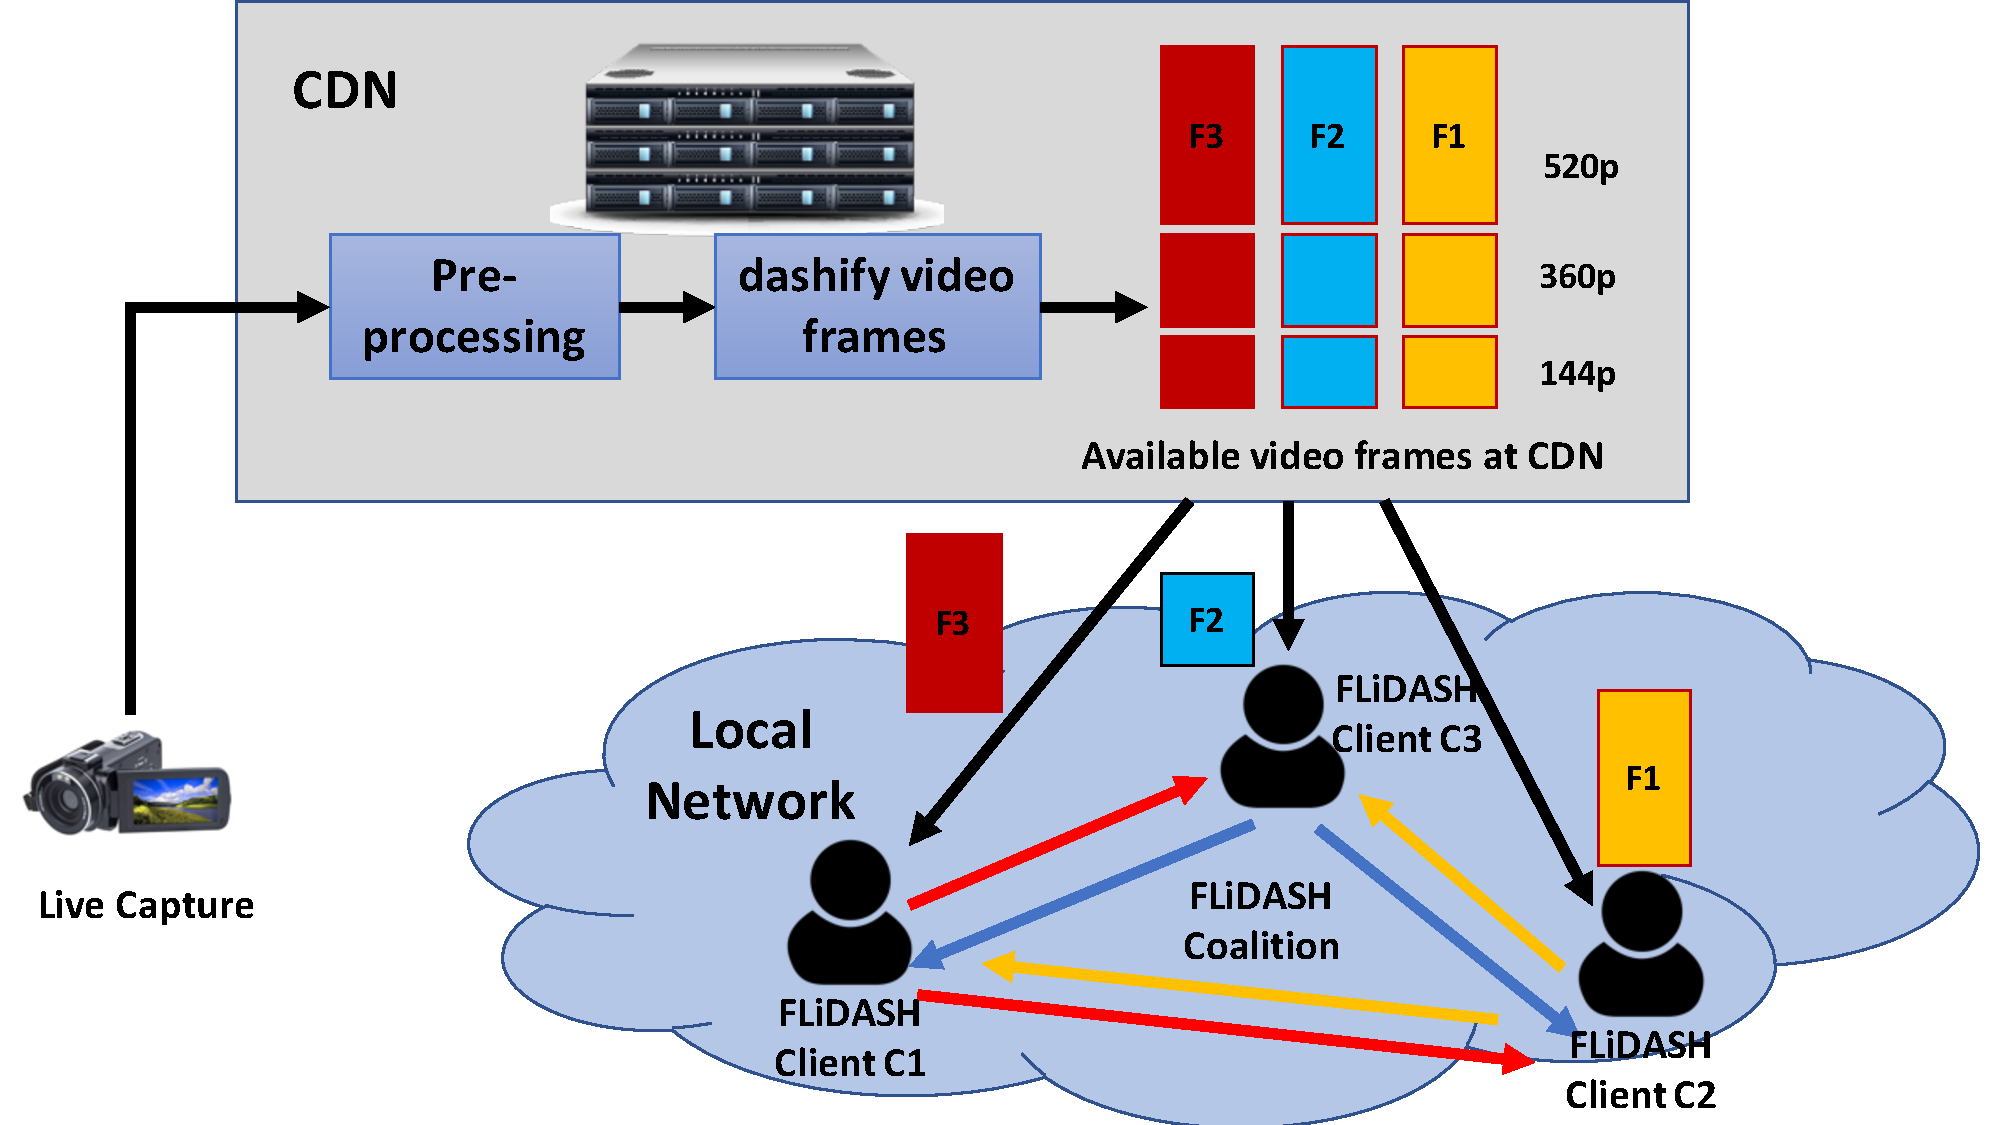
\includegraphics[width=0.8\linewidth]{img/flsd.pdf}
    \caption{Overview of \our: The clients under a local network create a coalition, every members of the coalition share the total download load.}
    \label{fig:chap06:flsd}
\end{figure}

However, developing such a system has multiple challenges. First, the coalition needs to be designed in a way such that downloading data directly from the content provider is costlier than sharing the data over the local network. Second, there should be a proper distribution of segment-wise data-download scheduling among the coalition members such that playback synchronization is not violated. A proper playback synchronization ensures that every player in the coalition should acquire the video segment $s_{i}$, either downloaded by itself or fetched from another coalition player through the direct local link, by the time it completes playing the previous video segment $s_{i-1}$; otherwise, there might be a rebuffering delay affecting the \ac{QoE}. Third, the Internet bandwidth of individual players may vary over time; therefore, the coalition as a whole should schedule the video segment downloads among its members as well as decide the bitrate of every video segment based on the \ac{ABR} principle.

Owing to the above challenges, we develop a coalition-based adaptive live streaming  called \textit{Federated Live Streaming over \ac{DASH}} (\our) where the streaming clients or players form a dynamic coalition based on the network quality parameters and collectively stream a live video. We use the playback buffer statistics at individual streaming clients to develop a distributed mechanism for coalition formation with the help from a proximity server (which can be an \ac{ALTO} server). The members of a coalition use a low-overhead gossip-based protocol for playback synchronization and takes following two decisions -- (1) scheduling the downloads of video segments among the coalition members based on their individual instantaneous network condition and the overall fairness criteria, and (2) bitrate of each video segments to optimize the overall \ac{QoE} of the coalition. We use the following \ac{QoE} objectives while making the above decisions -- (a) improve the overall video quality level, (b) improve the playback smoothness by reducing the quality fluctuations, (c) reduce rebuffering, and (d) improve fairness  among the coalition members in terms of the downloaded data share. We have implemented {\our} over an emulated environment and have thoroughly compared its performance with various other baselines. We observe that {\our} improves the overall \ac{QoE} with less traffic overhead at the backbone network.

The rest of the chapter is organized as follows. 

%   \setcounter{page}{1}
   \section{Related Work}
\acrshort{tcp} have two basic problems. 1) \acrshort{tcp} is tightly coupled with \acrshort{ip}, 2) \acrshort{tcp}'s slow-start mechanism is ill suited for short-lived connection. 
To solve the first problem. i.e. decoupling \acrshort{tcp} and \acrshort{ip}, first approach is to solve it from network. So, we got Mobile IP, \acrfull{hip}, \acrfull{shim6}. These protocols try to hide the information that underlying path has been changed. It \acrshort{tcp}'s congestion control suffers from this.

Another approach is to solve it from transport layer. For this we got \acrfull{sctp} and \acrfull{mptcp}. \acrshort{sctp} is similar to \acrshort{tcp}, but it provide multi-homing and multi-path for more reliability. It is not used because it is doesn't support \acrfull{nat} well. Application needed add support for this protocol. It wasn't drop in replacement for \acrshort{tcp}. \acrshort{mptcp} is drop-in replacement for \acrshort{mptcp}. It is almost traneparent to the application. If operating system support \acrshort{mptcp}, any exisiting application can start using \acrshort{mptcp}.


%   \setcounter{page}{1}
   \section{Motivation Behind the Research Work}

MPTCP is the most widely explored alternative for TCP, which supports multiple paths through multiple interfaces, while providing TCP like congestion control and reliability features for end-to-end connection. As mentioned earlier, a large number of researches~\cite{oh2016feedback,barik2016lisa,khalili2013mptcp,kheirkhah2016mmptcp,kheirkhah2015short} have explored MPTCP as an alternative of TCP for various application and network scenarios. However, MPTCP has two major shortcomings that prevent its large scale deployment over the Internet -- (a) MPTCP is implemented as a part of the Linux kernel, and therefore requires device reconfiguration for its deployment; and (b) MPTCP is still under exploration phase, and there are multiple shortcomings of MPTCP as pointed out by existing researches. In~\cite{khalili2013mptcp}, Khalili \textit{et al.} have claimed that MPTCP is not pareto optimal. Further, in~\cite{kheirkhah2016mmptcp}, the authors have pointed out that MPTCP is not suitable for short connections. 

Here, we first explore whether we can develop a MPTCP like protocol, or augment MPTCP so that we can support better network utilization for short flows. For this, we ask the following question: \textit{Why does MPTCP perform poorly for short flows?}  To get the answer, we do an emulation setup with the help of \texttt{Mininet} environment~\footnote{\url{http://mininet.org/} (last accessed: 24 April 2017)}, where we setup a network with two multi-homed hosts, and two distinct paths between the two hosts. We vary the end-to-end latency for the two paths, and then transfer data between the two hosts. For our experiment, we have configured the Linux kernel of the hosts with MPTCP version 0.91~\footnote{\url{http://multipath-tcp.org/} (last accessed: 24 April 2017)}. For this experiment, we set the path bandwidth as $50$ Mbps for both the paths. Among the two hosts, one host acts as the MPTCP server, while the other works as the MPTCP client. We keep a file at the server, and download that file from the client through MPTCP based connection. To observe the MPTCP behavior for various connection types, we vary the size of the file, and measure the impacts. 
%
%\begin{figure*}[ht]
%	\captionsetup[subfigure]{}
%	\begin{center}
%		\subfloat[\label{fig:percentSentOverPathRTT80}RTT=80ms]{
%			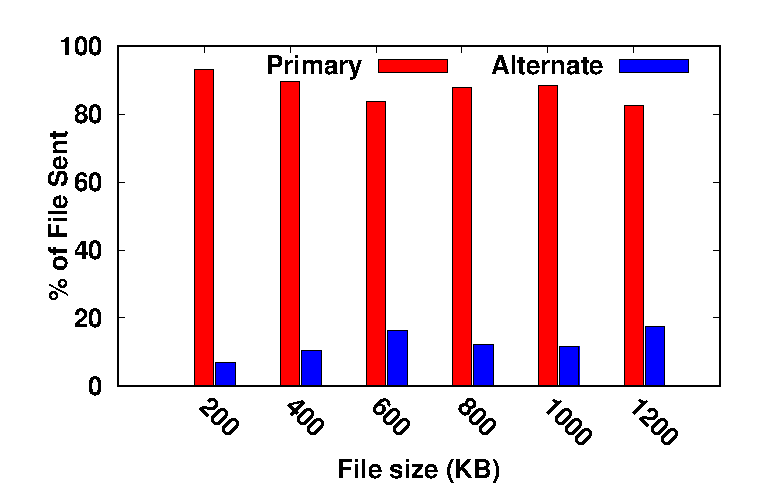
\includegraphics[width=0.32\linewidth]{img/exp4/delay-5}
%		}
%		\subfloat[\label{fig:percentSentOverPathRTT160}RTT=160ms]{
%			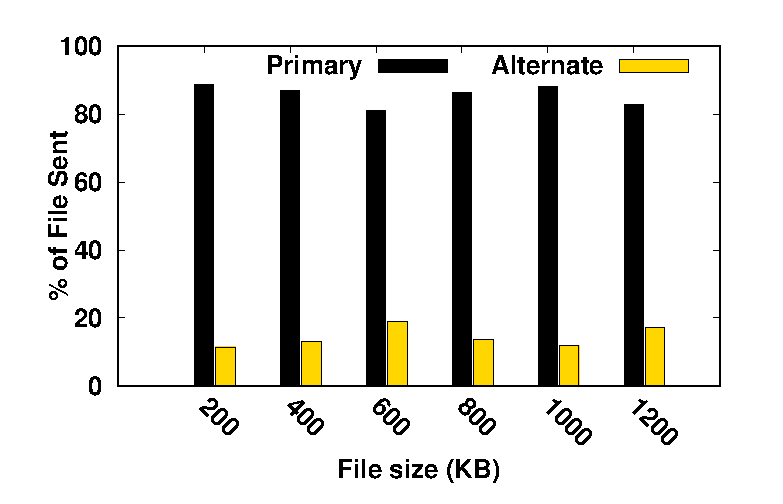
\includegraphics[width=0.32\linewidth]{img/exp4/delay-10}
%		}
%		\subfloat[\label{fig:percentSentOverPathRTT320}RTT=320ms]{
%			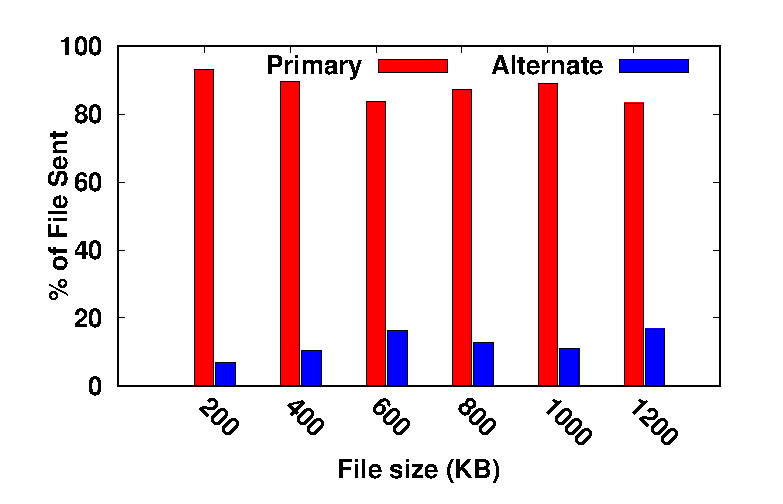
\includegraphics[width=0.32\linewidth]{img/exp4/delay-20}
%		}
%		
%		\caption{\label{fig:percentSentOverPath}\% of data share of a path.}
%	\end{center}
%\end{figure*}

\begin{figure}[!t]
	\begin{center}
	\begin{minipage}{0.45\linewidth}
		\centering
		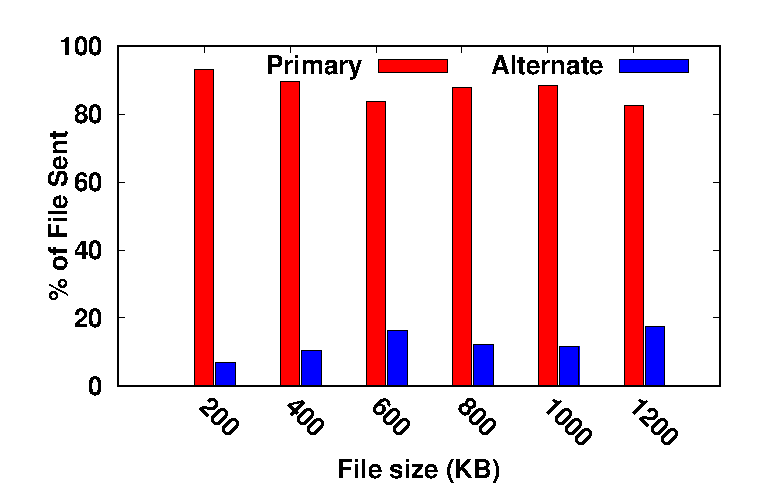
\includegraphics[width=\linewidth]{img/exp4/delay-5}
		\label{fig:percentSentOverPathRTT80}
		\subcaption{RTT=80ms}
	\end{minipage}
	\begin{minipage}{0.45\linewidth}
		\centering
		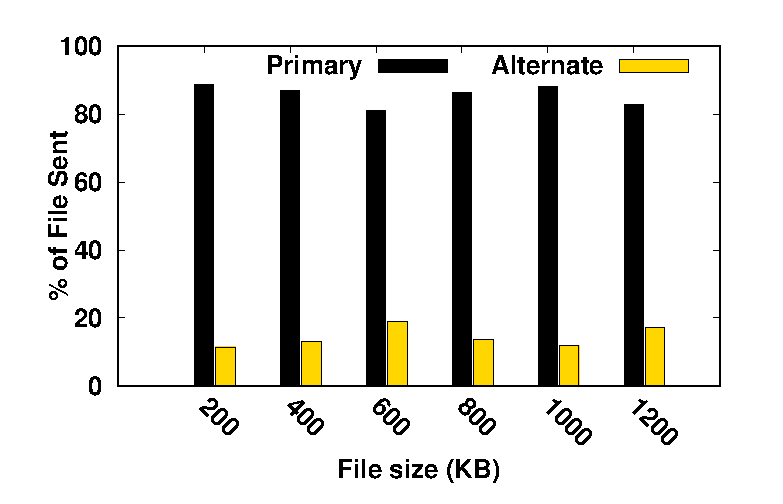
\includegraphics[width=\linewidth]{img/exp4/delay-10}
		\label{fig:percentSentOverPathRTT160}
		\subcaption{RTT=160ms}
	\end{minipage}
	\begin{minipage}{0.45\linewidth}
		\centering
		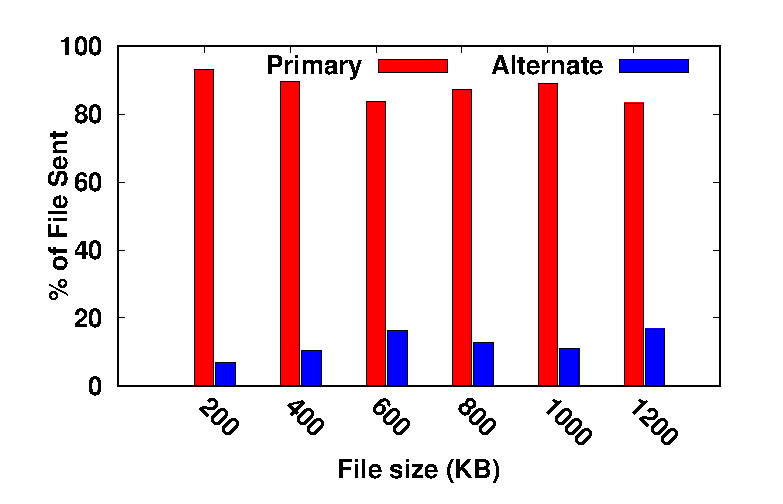
\includegraphics[width=\linewidth]{img/exp4/delay-20}
		\label{fig:percentSentOverPathRTT320}
		\subcaption{RTT=320ms}
	\end{minipage}
	\caption{\label{fig:percentSentOverPath}Percentage of Data Share between the Primary and the Alternate Paths}
	\end{center}
\end{figure}


\subsection{Utilization of Network Bandwidth at Alternate Paths for Short Flows}
MPTCP first initiates the connection through one of the available paths, called the {\em primary path}, and then explores the {\em alternate paths} to initiate alternate connections through them. In the first experiment, we try to look into the amount of data shares between the primary path and the alternate path. For this, we keep the bandwidth and latency for both the paths same, and vary the flow duration by increasing the size of the file to be downloaded at the client from the server. The results are plotted in Fig.~\ref{fig:percentSentOverPath}. We can observe from that figure that there is a huge imbalance between the two paths in terms of data share. The primary path forwards significantly more data compared to the alternate path. By exploring the connection logs, we find that by the time MPTCP sets up a connection to the alternate path, most of the data for a short flow has been transferred over the primary path. Further, the congestion controls for the primary and the alternate paths are handled separately, and therefore the alternate path also needs to go through the slow start phase. Therefore, the alternate path gets severely underutilized for short flows. Further, none of the primary sub-flow (sub-flow over the primary path) and the alternate sub-flow (sub-flow over the alternate path) can reach to the steady state for a short-lived flow.   

%
%We send the different sizes of data over from a host to another host via two separate paths in Mininet, where overall bandwidth and delay in the links are same for both the path. We find out that data share between two paths is imbalanced. We plot the results in Fig.~\ref{fig:percentSentOverPath}. We can see that 80\%-90\% of the data carries by primary path because \acrshort{mptcp} starts secondary sub-flow only after the establishment of the primary connection. By the time, secondary sub-flows establishes connection, primary sub-flow already sent several packets over the network. Primary sub-flow stays at least one \acrshort{rtt} ahead of secondary sub-flow. And none of the flow can reach the steady state for are short-lived flows.
%
%\acrshort{mptcp} can not balance between the different path for short-lived connection.

\subsection{Impact of MPTCP Path Selection During Connection Initiation}
We the perform another experiment on path selection, where the two paths have different round trip time (RTT). Here, we explore the effect of primary path selection, where we ask the following questions -- (a) {\em Does the RTT difference between the primary and the alternate path impact MPTCP performance?}; and (b) {\em Does the MPTCP performance differ if the low RTT path is selected as the primary path?} Consequently, we vary the RTT of the two paths, and the results are plotted in Fig.~\ref{fig:timeSentOverPath}. The two different bars in the graphs show the average file download time for two cases --  (i) low RTT path is used as the primary path, and (ii) high RTT path is used as the primary path. We observe that for small size file download, the performance varies a lot based on the selection of the primary path. However, the primary path selection is not a part of the core MPTCP mechanism, and MPTCP uses the path to set-up the primary sub-flow, which is provided by the underlying routing algorithm.  

%i.e. if \acrshort{mptcp} select longer path as primary path vs. shorter path as the primary path. In this experiment, we find that the time requires to send data using \acrshort{mptcp} over multiple paths largely depends on the primary path selection. For short-lived data and high RTT (Fig.~\ref{fig:timeSentOverPathRTT160}, Fig.~\ref{fig:timeSentOverPathRTT320}), it is taking significantly lesser time if \acrshort{mptcp} select shorter path as primary path. Results are plotted in Fig.~\ref{fig:timeSentOverPath}.
%\notesc{Do not use short and long paths -- use low RTT path and high RTT path in the figure. Use `File Size' instead of `Data Size'; and `Time Required to send Data' to `File Download Time'. }

%\begin{figure*}[ht]
%	\captionsetup[subfigure]{}
%	\begin{center}
%		\subfloat[\label{fig:timeSentOverPathRTT80}RTT: short path=80ms, long path=120ms]{
%			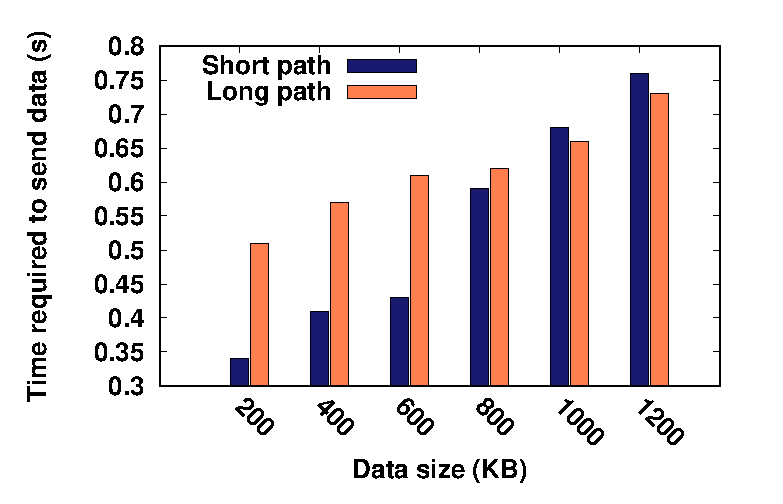
\includegraphics[scale=0.45]{img/exp5/time_needed_5}
%		}
%		\subfloat[\label{fig:timeSentOverPathRTT160}RTT: short path=160ms, long path=240ms]{
%			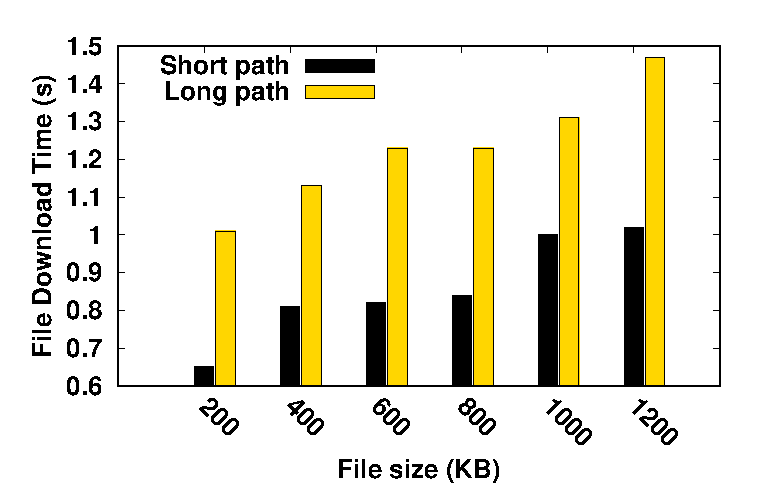
\includegraphics[scale=0.45]{img/exp5/time_needed_10}
%		}
%		\subfloat[\label{fig:timeSentOverPathRTT320}RTT: short path=320ms, long path=480ms]{
%			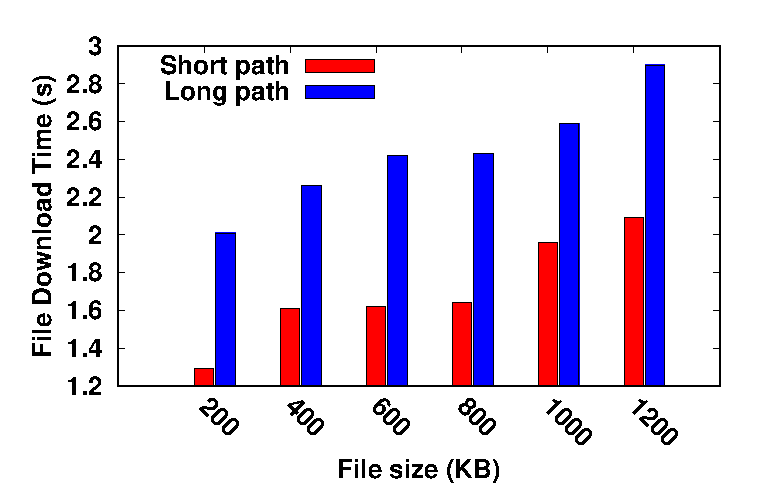
\includegraphics[scale=0.45]{img/exp5/time_needed_20}
%		}
%		
%		\caption{\label{fig:timeSentOverPath}Send data from client to server over 2 path using MPTCP. This is plot of \% of data went through a channel.}
%	\end{center}
%\end{figure*}

\begin{figure}[!t]
	\begin{center}
		\begin{minipage}{0.45\linewidth}
			\centering
			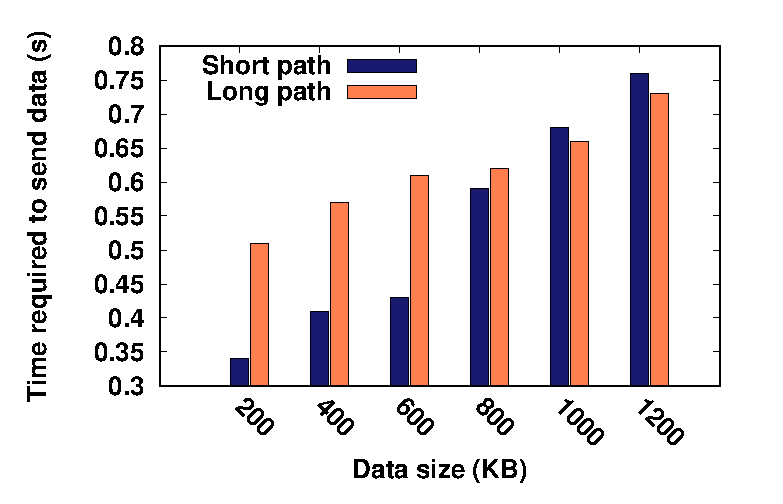
\includegraphics[width=\linewidth]{img/exp5/time_needed_5}
			\label{fig:timeSentOverPathRTT80}
			\subcaption{Short Path RTT: 80ms, Long Path RTT: 120ms}
		\end{minipage}
		\begin{minipage}{0.45\linewidth}
			\centering
			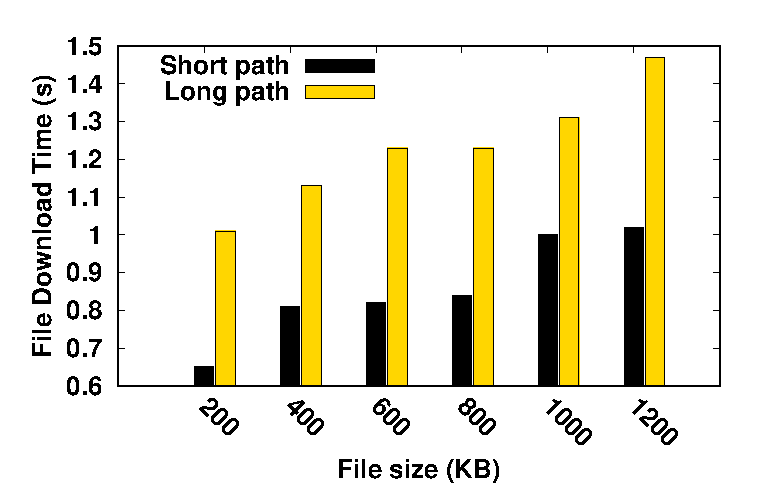
\includegraphics[width=\linewidth]{img/exp5/time_needed_10}
			\label{fig:timeSentOverPathPathRTT160}
			\subcaption{Short Path RTT: 160ms, Long Path RTT: 240ms}
		\end{minipage}
		\begin{minipage}{0.45\linewidth}
			\centering
			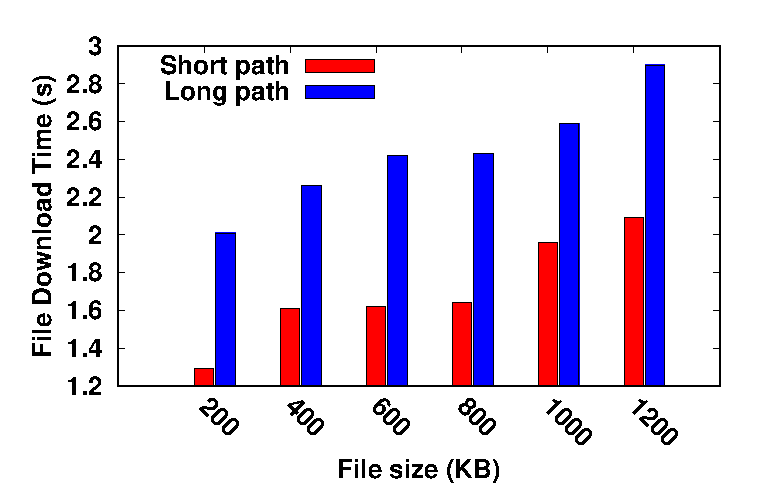
\includegraphics[width=\linewidth]{img/exp5/time_needed_20}
			\label{fig:timeSentOverPathRTT320}
			\subcaption{Short Path RTT: 320ms, Long Path RTT: 480ms}
		\end{minipage}
		\caption{\label{fig:timeSentOverPath}Difference in File Transmission Time based on the Primary Path Selection. The short path indicates the path with the low RTT value, whereas the long path indicates the path with the high RTT value}
	\end{center}
\end{figure}

%\acrshort{mptcp} is incapable of utilizing better path for short-lived connection if it makes mistakes in primary path selection. To overcome these issues and to use multipath, we developed \acrshort{udp} based multi-flow multipath protocol \textbf{Viscous}.
%
%In next section, we describe the protocol and how we overcome the problems with \acrshort{mptcp}.

\subsection{Take Aways}
In summary, the lessons learnt from the above experiments are as follows.
\begin{enumerate}
	\item Connection establishment time is an overhead for short flows. Further flow based congestion control algorithms results in the underutilization of network bandwidth, because every transport layer flow independently increases its transmission rate from the scratch (by increasing the congestion window value for TCP or MPTCP), and the flow may end before its transmission rate reaches to the network capacity. Flow multiplexing at the source device is important to handle such scenarios, however the HOL blocking problem needs to be avoided. 
	\item Connection establishment and path selection cannot be independent for a multi-path protocol, because the performance depends on the path selection mechanism. We need to develop a mechanism where the data transmission can be initiated simultaneously at multiple paths.   
\end{enumerate}
Accordingly, we target to develop a new transport wrapper as a part of this research, that works as a middleware between the application and the transport layer, and provides ubiquitous data transmission between two end hosts while ensuring reliability, flow control and congestion control.  The targeted protocol should use UDP as the transport protocol, and build up the services on top of that. 
%The detailed design philosophy of Viscous along with protocol specifications are discussed in the next section. 

\newpage 
%   \setcounter{page}{1}
    \section{Viscous: Protocol Descriptions}
To overcome the limitations of existing transport layer protocols as discussed in the previous section, we propose a new transport protocol called Viscous. It is a connection oriented multipath multi-flow transport protocol which is not coupled with the network stack, and work as a wrapper or a middleware between the users' application and the transport layer of the network protocol stack. The basic design philosophies for Viscous are as follows. 
\begin{enumerate}
	\item To mitigate the signaling overhead associated with connection establishment, Viscous multiplexes multiple flows over a single Viscous connection. This reduces the connection setup time for short-lived flows. 
	\item Viscous does not maintain a separate and independent congestion control for every application flows. Rather, it maintain a single congestion control mechanism for a Viscous connection which is a multiplex of multiple flows. Further, the congestion control is path specific, that is, congestion is monitored at every path from a source to a destination, where a Viscous sub-flow is initiated.  
	\item Viscous follows a modular architecture for ease development of applications. Any Viscous module can be tuned independently to make it suitable for a specific performance bound. This way, application layer quality of service (QoS) can be provided with the help of Viscous. 
	\item Viscous works on top of UDP, similar to Goggle's QUIC; therefore it mitigates the transport layer protocol overhead which is associated with TCP. 
	\item Viscous supports different types of mobility without breaking an existing connection. With the help of a unique client and server specific identifier which is shared during the initial connection establishment, Viscous can continue with the existing connection, even if the server or the client changes its IP address.   
	\item Viscous follows a layered architecture with two different layers, as shown in Fig.~\ref{fig:sys-io}. The top layer consists of multiple flows from various applications, and the bottom layer consists of multiple channels, corresponding to each path between a server and a client. To avoid the signaling overhead from the connection establishment and the slow-start phase, congestion control and reliability are associated with the bottom layer which consists the channels. On the other hand, flow-control and data transmission are designed as a part of the upper layer, which is associated with the flows.
	\item Consequently, Viscous decouples the congestion control from the flow control. This helps in avoiding slow start for all the flows between a source and a destination, those share common paths end-to-end. The flow control is kept flow specific, whereas the congestion control is kept channel or path specific. 
\end{enumerate}



\begin{figure}[!ht]
	\centering
	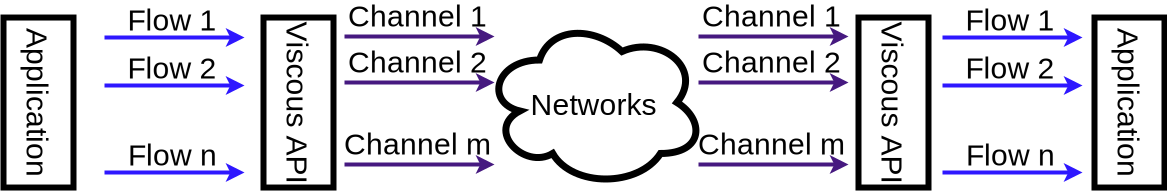
\includegraphics[width=\linewidth]{img/sys-io}
	\caption{Flow-Channel architecture in the Viscous protocol. Application sends and receives data through the flows. Internally, Viscous sends and receives data using multiple channels over multiple paths.}
	\label{fig:sys-io}
\end{figure}



%\acrshort{tcp} suffers for short-lived flow because of slow-start and connection establishment time. To mitigate this problem, we multiplexed multiple flows over a single viscous connection similar to \acrshort{quic}. 

%
We develop Viscous as a software library for Unix type systems. We implemented the entire protocol in the user space, and therefore we do not require any change in the existing Kernel or the TCP/IP protocol stack. In this section, we first discuss the fundamental concepts behind the development of Viscous and then talk about various internal protocol details for Viscous implementation.
%
\subsection{Key Concepts Behind the Design of Viscous}
There are two key concepts behind the design, development, and implementation of Viscous to support ubiquitous transport of data over any Internet devices -- \textit{flow} and \textit{channel}. These two concepts are the input and the output of the Viscous module, as depicted in Fig.~\ref{fig:sys-io}.

\subsubsection{Channel}
Channels are individual connections between two devices over multiple paths. There is one single channel for each path. To avoid connection time path imbalance like MPTCP, as we observe in Fig.~\ref{fig:timeSentOverPath}, we initiate all the channels simultaneously after connection establishment and before any flows can start. Connections are established specific to a destination host whenever an application from a source host requests for a connection. This connection is shared with other applications which intend to send data to the same destination host. This way, flows are multiplexed specific to a destination host. A common example for such scenario is the IoT gateway applications, where multiple sensor nodes transfer data to a destination gateway via a common source gateway. In Viscous, flows do not require connection establishment as the connection has already been established between the source and the destination. Viscous handles congestion control for every individual paths between a source and a destination. Therefore, flow specific congestion control is not required for Viscous, and Viscous maintains path specific congestion control. This way Viscous avoids slow start for every individual flows that share the complete path from the source to the destination. Consequently, channels are persistent in Viscous, and they do not die out after the completion of a flow. As mentioned, a channel can carries data from multiple flows simultaneously by multiplexing them. If one or both the devices are multi-homed, multiple channels can be established that share the traffic load and therefore, achieve better performance.

\subsubsection{Flow} 
Flows in Viscous are responsible for data communication while maintaining the flow-control between a source and a destination. An application can transmit data over multiple flows simultaneously. The user application sends data as byte-streams to the flow, and it also receives data in the form of byte-streams from a flow. Flow is responsible for packetizing the byte-stream and sending the packets to the lower layer of Viscous. We do not put congestion control inside a flow because it is not persistent and we do not want to go through the same slow-start phase again for multiple flows between a source and a destination. So, Viscous puts packets from flows to channels, and the channels take care of the congestion control. This way, we decouple congestion control from flow control in Viscous design. 

This channel-flow decoupled architecture gives Viscous the power of utilizing multiple paths even for short-lived flows. Flows do not have to suffer from slow-start or connection establishment overhead. The connection establishment is a separate event from channel management, and all the channels between a source and a destination start simultaneously. This removes the problem of path selection as we observe in MPTCP.  Further, channel gives an option to support mobility. If one or both the devices change its network address, the associated channel cannot communicate anymore. Viscous can discard the affected channels and initiate new channels using the new network address without any interruption in Viscous connection (application flows). 


\subsubsection{Channel Scheduler}
Viscous channel scheduler schedules packets from application flows to one of the channels. A straightforward way  to schedule the packets is to allocate channels to the packets in a round robin way. However, round robin channel scheduling is not optimal because different channels can have different network characteristics in terms of bandwidth, delay or packet loss; as they are associated with different end-to-end paths in the network. Therefore we use an acknowledgement (ACK) driven scheduling for Viscous, that works as the base scheduler. Here the scheduler schedules a packet to a channel when it receives the ACKs corresponding to the already transmitted packets in the channel. Whenever the scheduler receives an ACK over a channel, it schedules the next packet to that channel. This provides a self-clocking behavior to the channel scheduler. This way, Viscous resolves the issue of balancing packets among various channels.

It can be noted that this is the base scheduler that we have designed for Viscous. The scheduler can be extended to support application QoS, where different flow may require different bandwidth. This provides design flexibility to Viscous, where an application programmer can control Viscous modules for applications' need.  

%The real power of Viscous lies in $flows$. An application will communicate with remote applicate using a flow only. The application can run multiple flows simultaneously without blocking other flows. Flow can start to send data without spending any time in connection establishment and may not have to go through the slow-start phase. Flows allow an application to transmit byte-stream from one application to remote application. Flows are responsible for packetizing byte-stream and send the packet to lower layer. It is also responsible for reordering unordered packets received from the lower layer and send byte-stream to the application. Flows are not liable for reliable transmission or congestion control as \textit{channel} handles these things. However, it should provide flow control mechanism.

%\subsubsection{Interface Id} Viscous mark every network interface available in a device by a 4-bit nonzero positive integer. For now, we only support maximum 15 interfaces (although never tested with 15 interfaces).

%\begin{figure}[!h]
%    \centering
%    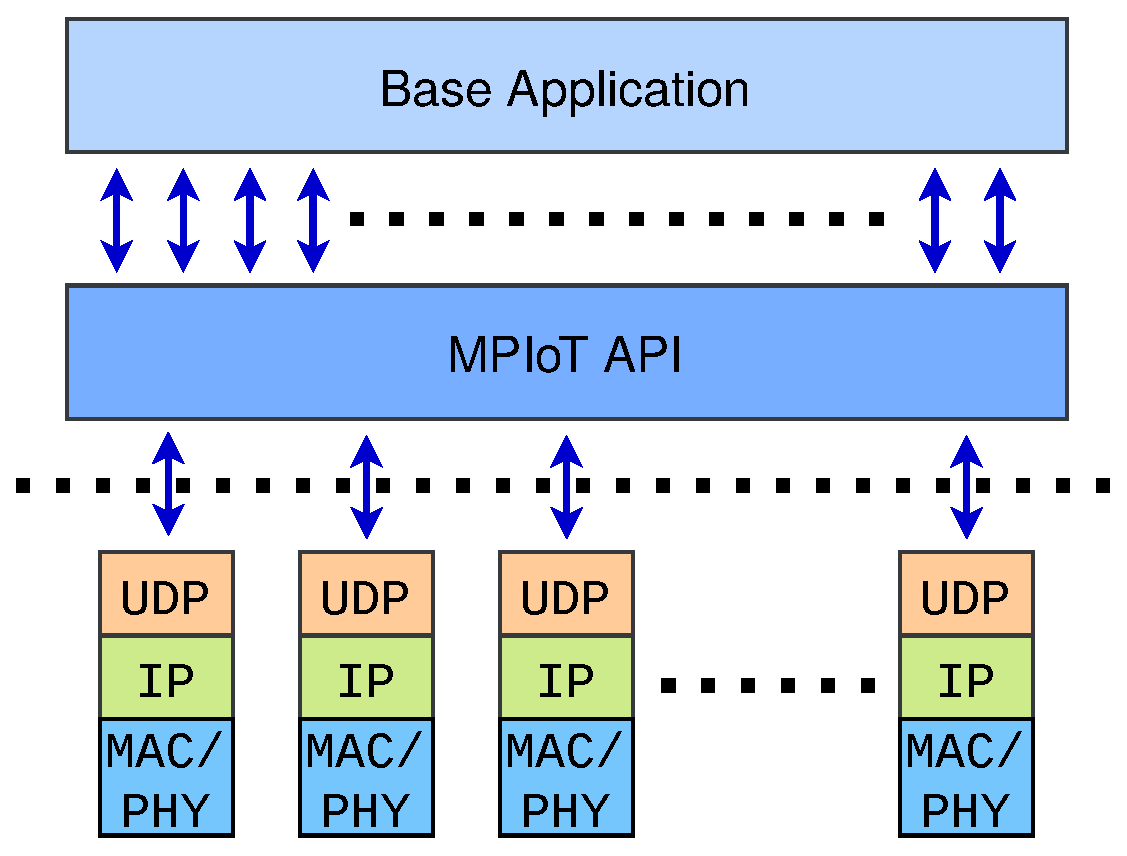
\includegraphics[width=.65\linewidth]{img/sysArch}
%    \caption{}
%    \label{fig:sysArch}
%\end{figure}


%\subsubsection{Channel} 
%Channel is an internal method Viscous uses to communicate to a remote Viscous enabled application. Flows are internally multiplexed and send through one or more channel. Each distinct source-interface and destination interface pair can one channel. Channels are expected to provide reliable transmission between two application. It is also responsible for handle congestion in the pipe. An application can not use channels directly to transmit data. Creation of channel is implementation dependent. There is no requirement of any handshaking during the channel creation. However, it is needed to check if a channel can be established or not. It may happen that, there is no path between one interface-pair.


Viscous is a connection oriented protocol. So it uses the client-server architecture for creating and maintaining the connections. A Viscous server waits for a new connection from a Viscous client. One Viscous server can stay and manage connections with multiple clients. For each client connection, the server maintains separate sets of channels and other associated modules. This separation of channels is required as the different clients may follow different paths from the server. 

%
%\subsubsection{Viscous Server}
%Similar to \acrshort{tcp} server, a viscous server waits for clients to connect to it. The client connects using three-way handshaking method similar to \acrshort{tcp}. 
%%
%\subsubsection{Viscous Client}





\subsection{Protocol Description}
Like every connection-oriented protocol, the life-cycle of Viscous also starts with the connection establishment state.
Other states of this protocol are -- ready to create flow,  ready to close, and  connection closure.
%Figure \ref{fig:ProtocolLifeTime} depict life cycle of viscous.
In Viscous, communication is possible only after association of the flows to the connections. Accordingly Viscous maintains the above four states as discussed next. Fig.~\ref{fig:ProtocolDiagram} shows the protocol diagram for Viscous. 

\begin{figure}[!ht]
	\centering
	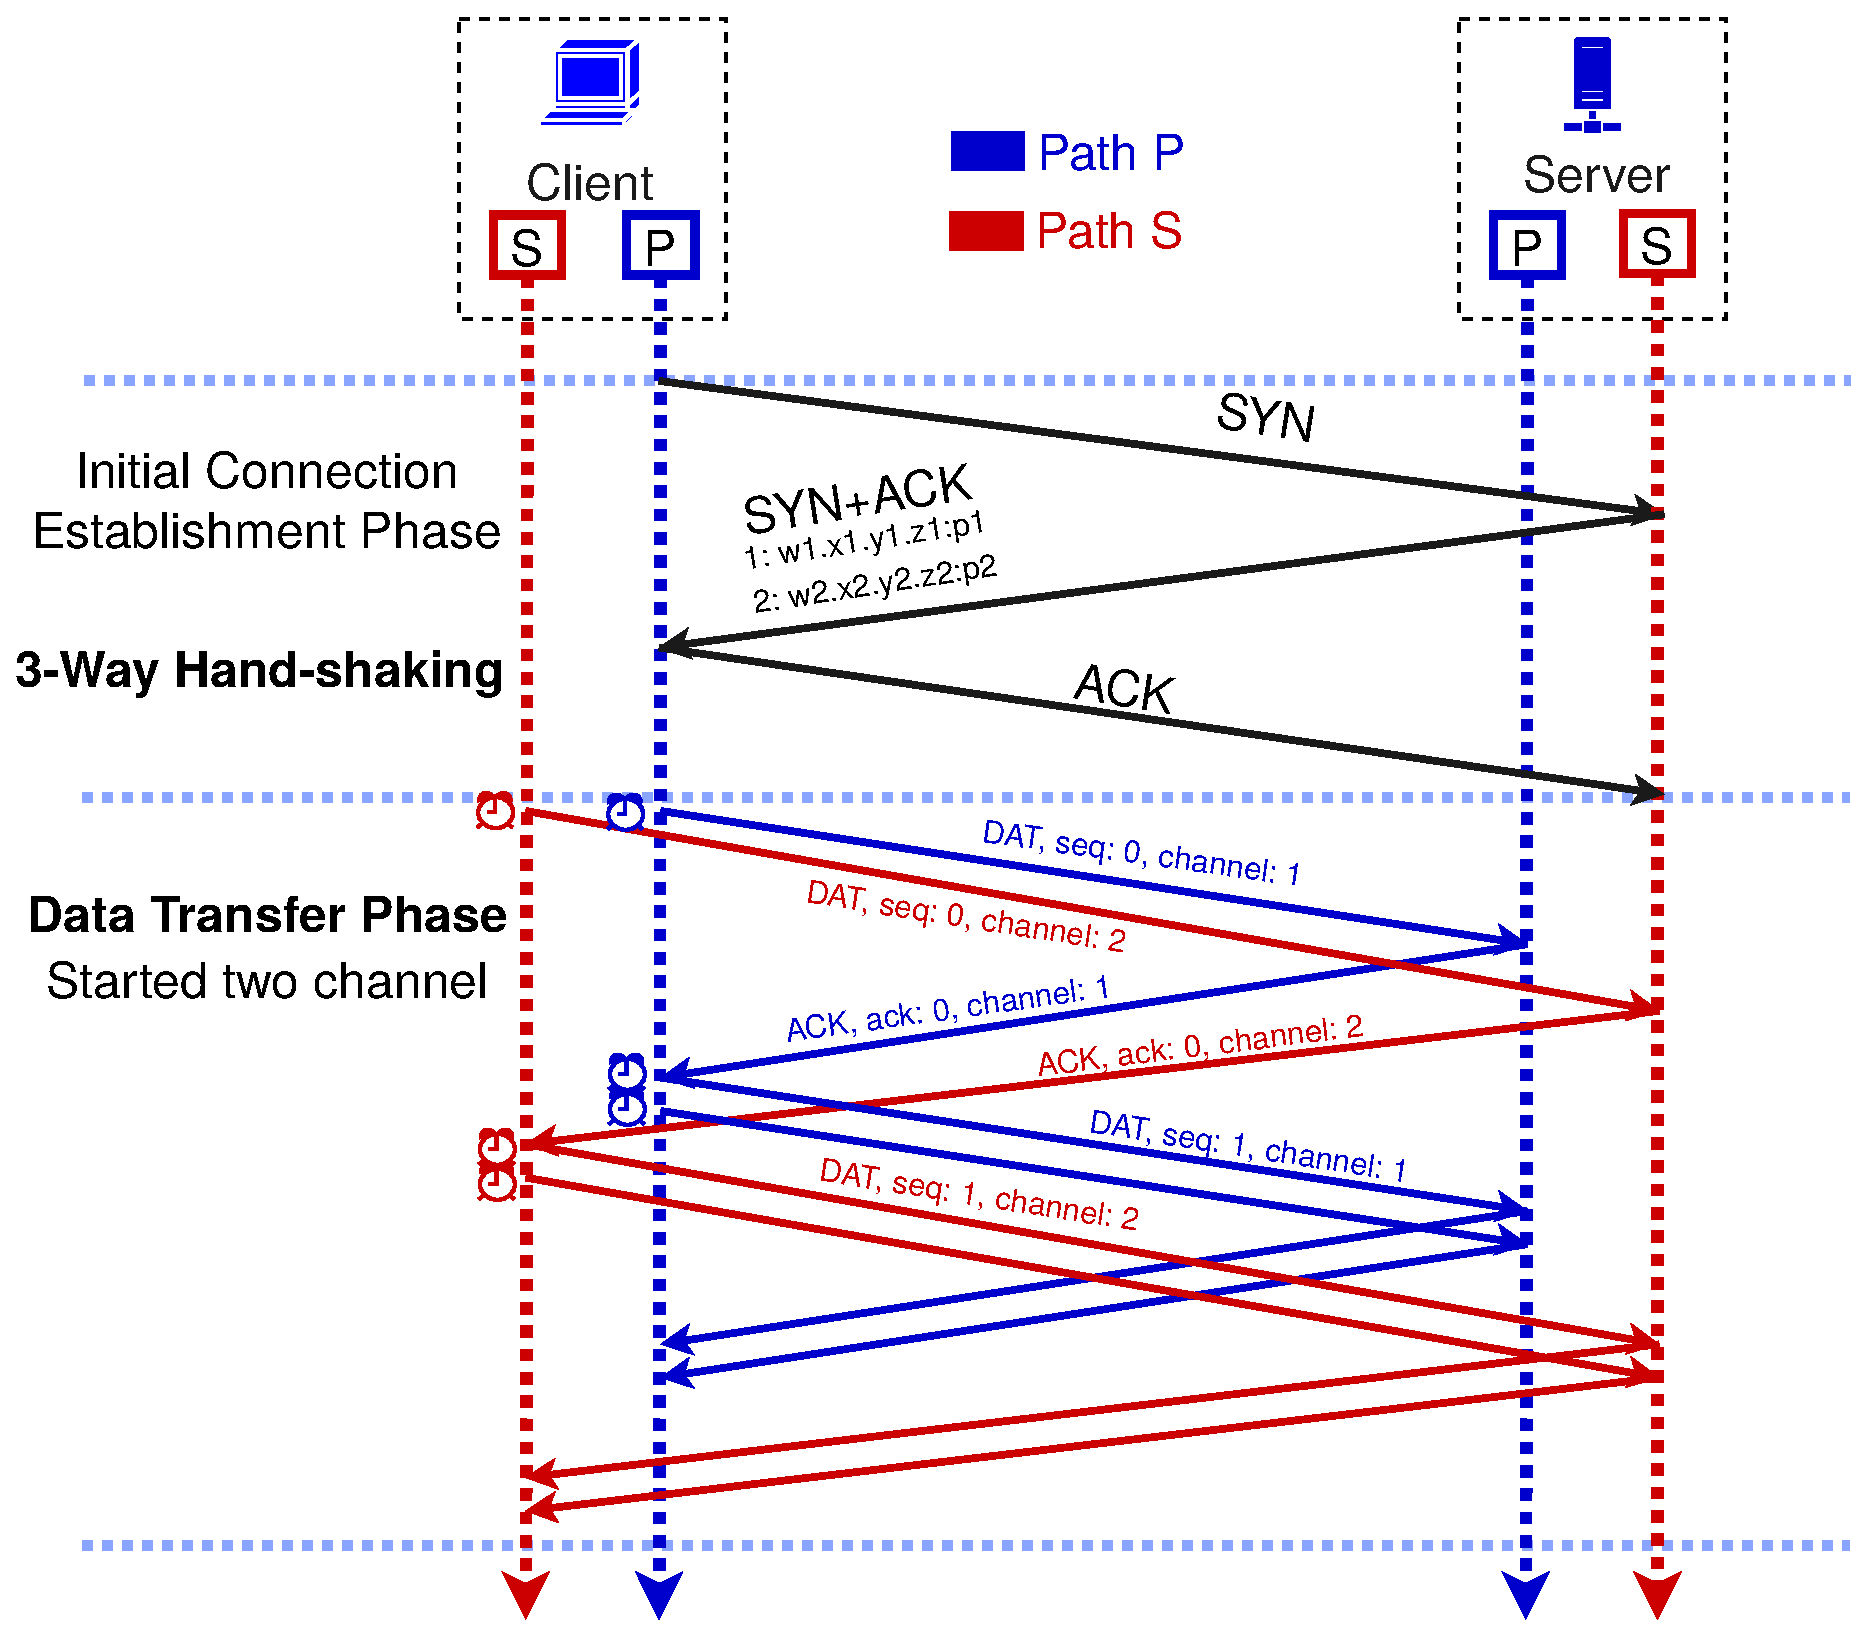
\includegraphics[width=1\linewidth]{img/ProtocolDiagram}
	\caption{Three way handshaking between client and server and data transfer between them. Handshaking can go between any two pairs of interfaces.}
	\label{fig:ProtocolDiagram}
\end{figure}

%\begin{figure}[!h]
%    \centering
%    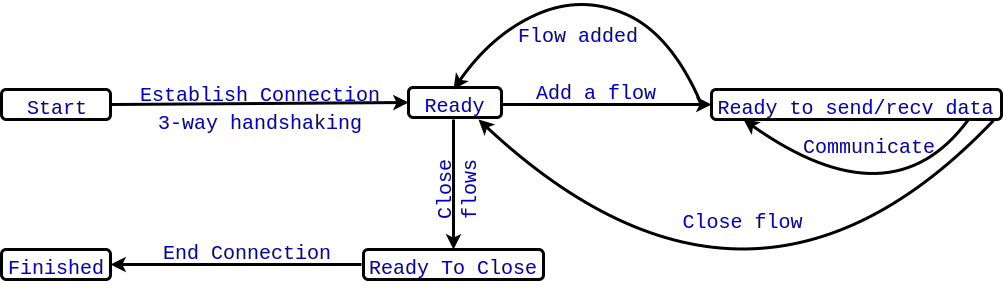
\includegraphics[width=1\linewidth]{img/ProtocolLifeTime}
%    \caption{}
%    \label{fig:ProtocolLifeTime}
%\end{figure}

\subsubsection{Connection Establishment}
We keep this procedure similar to the TCP connection establishment procedure that follows a three-way handshaking mechanism. However, as mentioned earlier, connection establishment in Viscous is in between a Viscous server and a Viscous client which is one time and does not depend on the number of flows between the same server-client pair. To establish a connection, the Viscous client sends a synchronization (\texttt{SYN}) packet with a temporary unique identifier. We can use the MAC address or the IP address of the client as this identifier. On receiving the \texttt{SYN} packet, the Viscous server generates a fingerprint for the client and sends a \texttt{SYN+ACK} packet containing the generated fingerprint. This fingerprint is used as the connection identifier for the server-client pair , and every packet between the server and the client includes this fingerprint. In our implementation, we use a SHA256 has function to generate the fingerprint from the client MAC, server MAC and the current time-stamp used as a unique nonce. It can be noted that different fingerprint is used for different connections, and therefore a fingerprint can uniquely identify a path between a server-client pair.  The connection establishment procedure ends with the Viscous client sending an \texttt{ACK} packet.
%\begin{itemize}
%    \item \textbf{SYN}: Synchronisation flag similar to \acrshort{tcp}. Indicate receiver that connection is being synchronized.
%    \item \textbf{ACK}: Acknowledgement flag. Indicator to the receiver that packet acknowledges previously received data or other packets.
%\end{itemize}

%The fingerprint is a unique identifier for a client generated by the server. 
%It is required in this protocol as this protocol can not use IP-Port tuple as client identification. 
%Viscous is a multipath protocol; each interface will have different IP-Port tuple.
%A fingerprint is the better way to identify connection when packets are going through various path/interface.
%
%Temporary unique identification is client's identification before it received any fingerprint. 
%It is required to identify a client in case of $SYN+ACK$ packet got lost, and client needs to resend the $SYN$ packet.
%We do not want to rely on this identifier for further communication because the client generates it, and any other clients may generate the same identifier by mistake or intention.

A packet loss during the connection establishment is detected using timeout. If ACK is not received within the predefined period after sending a \texttt{SYN} packet, the sender (client or server) retransmits the packet again. In our implementation, we use a timeout value of $1$ second for retransmitting a \texttt{SYN} packet, and a device can retry up to three times. During the connection establishment, the Viscous server informs all its network addresses to the Viscous client, if the server has multiple interfaces. So, immediately after the connection establishment at one channel, the Viscous client initiates all possible channels to the Viscous server. There is no requirement to send an extra control packet to complete the channel establishment. 
%Channel establishment will automatically complete when server side receives first packets of a channel from a client.
After connection establishment, Viscous clients become ready to add flows to the channels, and initiates the data transmission as the applications send data over the flows.

\subsubsection{Ready State}
Once connection got established, bothe the Viscous client and the Viscous server become ready to transmit or receive data by creating flows from the applications. We say that the Viscous protocol is under \textit{Ready} state at this phase. In this state, the Viscous channel scheduler schedules flows to the channels based on data generation from the application. 

\subsubsection{Connection Closure}
When an application has finished all the transmissions with the remote application, the application can close the Viscous connection. Connection closure in Viscous is implementation dependent, and we use TCP type connection closure at every channel that was established between the server and the client. 

\begin{comment}
\subsection{Layers in Viscous}
The Viscous protocol has multiple layers. Each layer is responsible for a different task. We are going to discuss each layer now in a top-down approach.
\subsubsection{Top layer or \acrshort{api} layer}
Top layer or \acrfull{api} layer is the layer when application directly interacts with Viscous protocol library. This layer defines how an application will interact with the protocol \acrshort{api}. It can be defined as application layer also.
\subsubsection{Flow layer}
Flows are defined in this layer. After connection establishment, an application will create one or more flows to transmit data. Data transmission between applications through flows is handled. This layer is responsible for flow control and packet reordering. There will be a multiplexer-demultiplexer at the bottom of this layer. This multiplexer-demultiplexer is liable multiplex packet arrived from different flows and sent to the lower layer and vice-versa.

\subsubsection{Channel scheduling layer}
When Viscous have multiple channels, it is needed to schedule packets to one of the multiple available channels. Channel scheduling layer responsible for this task. It is one of the important layers. Scheduling job is critical. An optimized schedulers can increase performance by reducing out-ordered packet, jitter, and delay. 

\subsubsection{Channel layer}
Channel layer is the most important layer in Viscous. This layer is responsible for taking a packet to remote device/application reliably, efficiently and equitably with other traffic in the network. This layer needs to handle congestion in a network. We do not suggest any new congestion control mechanism. \acrshort{tcp} provides multiple congestion control algorithm. Implementation can borrow any congestion control algorithm from \acrshort{tcp} and implement here. One of the important tasks of the channel layer is sent a packet through proper interface. How does an implementation can send a packet through an interface is implementation dependent. The only requirement here is, a channel should be able to forward packet to predecided particular interface and packet should reach a pre-decided specific interface at the remote device. To do this implementation may add one more layer to handle interface.

Novelty in our protocol approach is that it does not suffer from head-of-the-line blocking problem. We achieved it by separating packet reordering, flow control and congestion control in two layers. Channel layer only takes care of the congestion control. It does not store any packet it receives. Instead, it just forwards them to flow layer. Channel only keep track of the received packet in the form of a bitmap to provide reliable data transmission.

The flow layer is responsible for packet reordering and flow control. The flow layer does it individually for each flow. So, if a packet loss for one flow, it does not affect other running flows.

%\begin{figure}[!h]
%\centering
%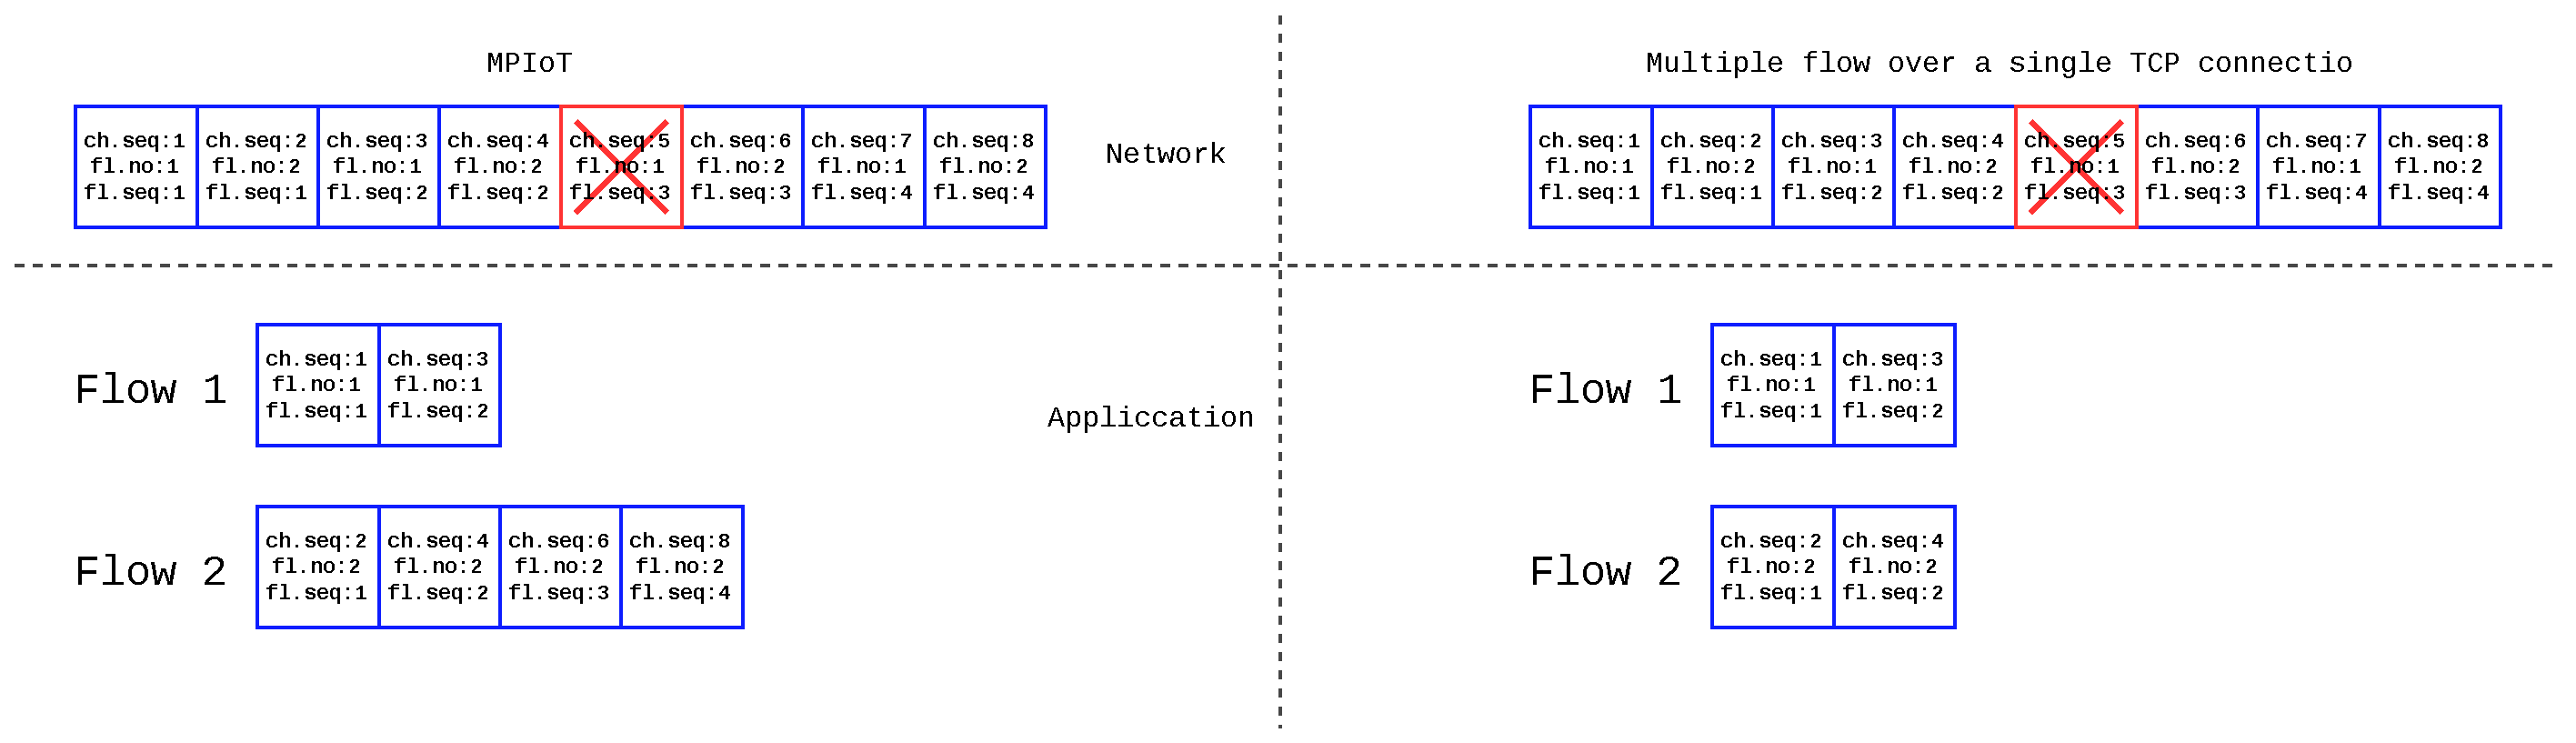
\includegraphics[width=\linewidth]{img/HOL-unblocked}
%\caption{}
%\label{fig:HOL-unblocked}
%\end{figure}


%In figure \ref{fig:HOL-unblocked}, we described how HoL blocking works for \acrshort{tcp}.
\end{comment}

\subsection{Mobility Support in Viscous}
Viscous can support different types of mobility events, as follows. 

\subsubsection{Connect-time Mobility}
A connection can fail whenever the server or the client changes its address in between the connection establishment time. With the help of a global name server, this type of mobility can be supported in Viscous. A name server is required to get the new address of the server, when the server changes its IP address. There are two cases that needs to be handled. 
\begin{enumerate}
    \item \textit{Client changes its address just after sending a \texttt{SYN} packet, Server changes its address just after receiving a \texttt{SYN} packet}: This type of failure is automatically recovered by subsequent retries from the client. During the retry, the Viscous client is identified via temporary unique identifier which is used to generate the fingerprint.
    \item \textit{Client or server changes its IP address after receiving the \texttt{SYN+ACK} packet from the server}: As \texttt{SYN+ACK} packet contains the fingerprint, the client can send the \texttt{ACK} packet to complete the three-way handshake by sending the \texttt{ACK} packet to the new server address. The new server address is received with the help from the global name server. However, the success depends on how fast the global name server can update the server IP address against its domain name. If this process fails after three retries, the client re-initiates the connection. 
\end{enumerate}

\subsubsection{Individual Mobility}
Individual mobility event occurs when one of the interfaces from both the devices change its network address. This type of mobility can affect a Viscous connection, only if the affected channel already has some packets under transmission. The subsequent packets will carry the new address to the remote device. This does not create a problem, because the connection is identified by the unique fingerprint between the server and the client. 

Further, the new IP address can be forwarded via other unaffected channels. If all the channel fails, the the affected application can take help from the name-server to find out the new address, and the new channels are creates based on that.

\subsubsection{Simultaneous Mobility}
Simultaneous mobility is rather complex, which occurs when all the interfaces of the server or the client change their network addresses simultaneously. In this scenario, the remote application is not reachable at all. In this event, all existing channels are affected. Therefore, the application needs to get the remote addresses from the name server. Once it get the new addresses, Viscous can continue with the existing connections as the fingerprint remains unchanged.

    \section{Viscous Implementation: Packet Structure and Protocol Modules}
We have implemented and tested Viscous using C++ language in Linux\footnote{Our implementation may not work in other Unix based kernel. There is some dependency from Linux kernel.} kernel environment with \texttt{pthread} library. 
In this section, we give the implementation details for Viscous. 

\subsection{Packet Structure}
Fig.~\ref{fig:packet_format} depicts the packet structure used in Viscous. The basic packet structure for Viscous is influenced by TCP packet structure. Each packet is divided into three parts -- a) {\em Mandatory Header}, b) {\em Variable Length Optional Headers} for additional information, and c) {\em Data Region}. The maximum size of a Viscous packet is based on the Maximum Transmission Unit (MTU) for the corresponding network. At the current implementation of Viscous, we do not allow segmentation. 

\begin{figure}[!ht]
    \centering
    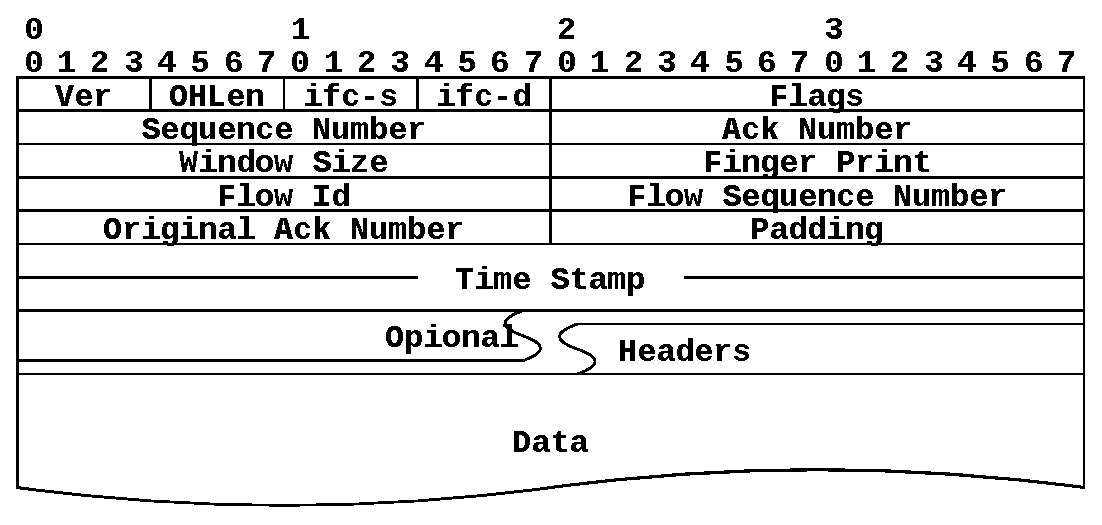
\includegraphics[width=0.75\linewidth]{img/Packet_format.eps}
    %\framebox[0.9\linewidth]{\input{img/Packet_format.tex}}
    \caption{Viscous packet header structure}
    \label{fig:packet_format}
\end{figure}

\subsubsection{Mandatory Header}
Every packet starts with $28$ bytes mandatory headers. Different fields in the mandatory header are as follows. 
\begin{itemize}
    \item \textbf{Ver}: $4$ bit protocol version number. The current version is 1.
    
    \item \textbf{OHLen}: $4$ bit optional header count. We can accommodate at most $16$ optional headers in a packet. As optional header size are different, it makes sense to store the number of optional headers than total size of it.
    \item \textbf{Ifc-s}: $4$ bit application defined source interface ID.
    \item \textbf{Ifc-d}: $4$ bit application defined destination interface ID. Each application can use the device and list down the interface IDs available. At the current implementation of Viscous, we assume that a device cannot have more than $15$ interfaces. Interface IDs start with $1$. Interface id $0$ (zero) means it is not a valid interface. In our implementation, we use a pair of local and remote interface IDs as the channel identifier. So, our implementation can support at most ($15\times15$) $225$ channels.
    \item \textbf{Flag}: Set of $1$ bit flags. We discuss it later in this section.
    \item \textbf{Sequence Number}: $16$ bit sequence number for a single packet. This sequence number is packet sequence number. In Viscous, we use packet based sequence number because of two reasons: a) packets are not created by the channel handler and b) As we multiplex multiple flows, it is easier to track a packet from a flow than an byte sequence from a flow. Sequence numbers are used by the channel handler to provide reliable communication between two applications. Two channels can have same sequence number for a packet.
    \item \textbf{ACK Number}: $16$ bit acknowledge number. In Viscous, we use cumulative acknowledgment number similar to TCP. It denotes that the receiver has received contiguous packets up to this sequence number, and it has not received the next packet until the time it was sent from the receiver.
    
    \item \textbf{Window Size}: Receiver's advertise window. This is used for flow control in Viscous. 
    
    \item \textbf{Fingerprint}: It is the client's unique ID generated by the server. Every packet includes this field except the \texttt{SYN} packet. In Viscous, packets are discarded silently if this field is 0 (zero) or if there are no connections that matches with the fingerprint (i.e. invalid fingerprint).
    
    \item \textbf{Flow ID}: We use a $16$ bit flow ID in Viscous. To keep implementation simple, we use a $16$ bit integer as the flow identifier.
    
    \item \textbf{Flow Sequence Number}: $16$ bit sequence number for each flow. It is independent of the packet sequence number. This parameter is required at the flow layer to reorder the packets at the receiver side. While the sequence number fields determine number of packets transmitted over a connection, the flow sequence number indicates the number of packets transmitted or received from a single flow. Because of the similar reason for using packet based sequence number, we also use packet based flow sequence number at the flow layer.
    
    \item \textbf{Original ACK Number}: Viscous uses selective acknowledge mechanism. When the receiver receives an out of order packet, it is supposed to send duplicate acknowledgment packets acknowledging the last conscious packet received. The receiver puts the original sequence number of the packet which triggers the duplicate acknowledgment. This field gives sender an indication about the packets received at the receiver side. So, the sender does not resend them again. It helps Viscous in reducing number of overall retransmissions.
    
    \item \textbf{Padding}: We use a $16$ bit padding to keep the header size in the power of $2$. This is currently an empty space in the header that can be reused later on. 
    
    \item \textbf{Sender Timestamp}: When a sender sends a data packet it includes a current Unix timestamp in microseconds ($\mu s$). When a receiver receives a data packets, it includes this timestamp with the ACK packet. It helps the sender in measuring the RTT more accurately.
\end{itemize}

\subsubsection{Flags in Viscous Mandatory Header}
In our implementation, we reserve $16$ bits for several $1$ bit flags. Although we can use $16$ different flags, currently we are using only eight flags. Fig.~\ref{fig:flags} gives an illustration of every flag and their position in bit fields. These flags are as follows. 

\begin{figure}[!ht]
    \centering
    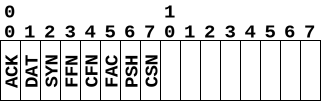
\includegraphics[width=.5\linewidth]{img/flags}
    \caption{Flags in Viscous Packet Header}
    \label{fig:flags}
\end{figure}

\begin{itemize}
    \item \textbf{$ACK$}: Acknowledgment flag that describes that the packet contains an acknowledgment number.
    \item \textbf{$DAT$}: Data flag. In our implementation, a packet goes up to the flow layer only, if the packet is marked as DATA packet.
    \item \textbf{$SYN$}: Synchronization flag used for connection establishment.
    \item \textbf{$FFN$}: Flow finished indicator. We use it to close a single flow.
    \item \textbf{$CFN$}: Connection/client finish flag. We use it for connection closure.
    \item \textbf{$FAC$}: Flow acknowledgment. 
    \item \textbf{$PSH$}: Push flag. It is the indicator that a flow has just started, i.e. this is the first packet of a flow.
    \item \textbf{$CSN$}: Channel Synchronization flag. It is being used when we try to set up a channel. It is the first packet that every channel sends to the other end. It is a two-way handshaking for channel establishment.
\end{itemize}


\subsection{Modules and Layers in Viscous Design}
We have developed several modules to perform different purposes throughout the lifetime of the Viscous protocol. These modules support application programmability, where an application developer can independently change a module without affecting others, based on the need from the application. The block diagram given in Fig.~\ref{fig:ProtocolDiagram} gives an elaborate description of our modular implementation of Viscous.

\begin{figure}[!ht]
    \centering
    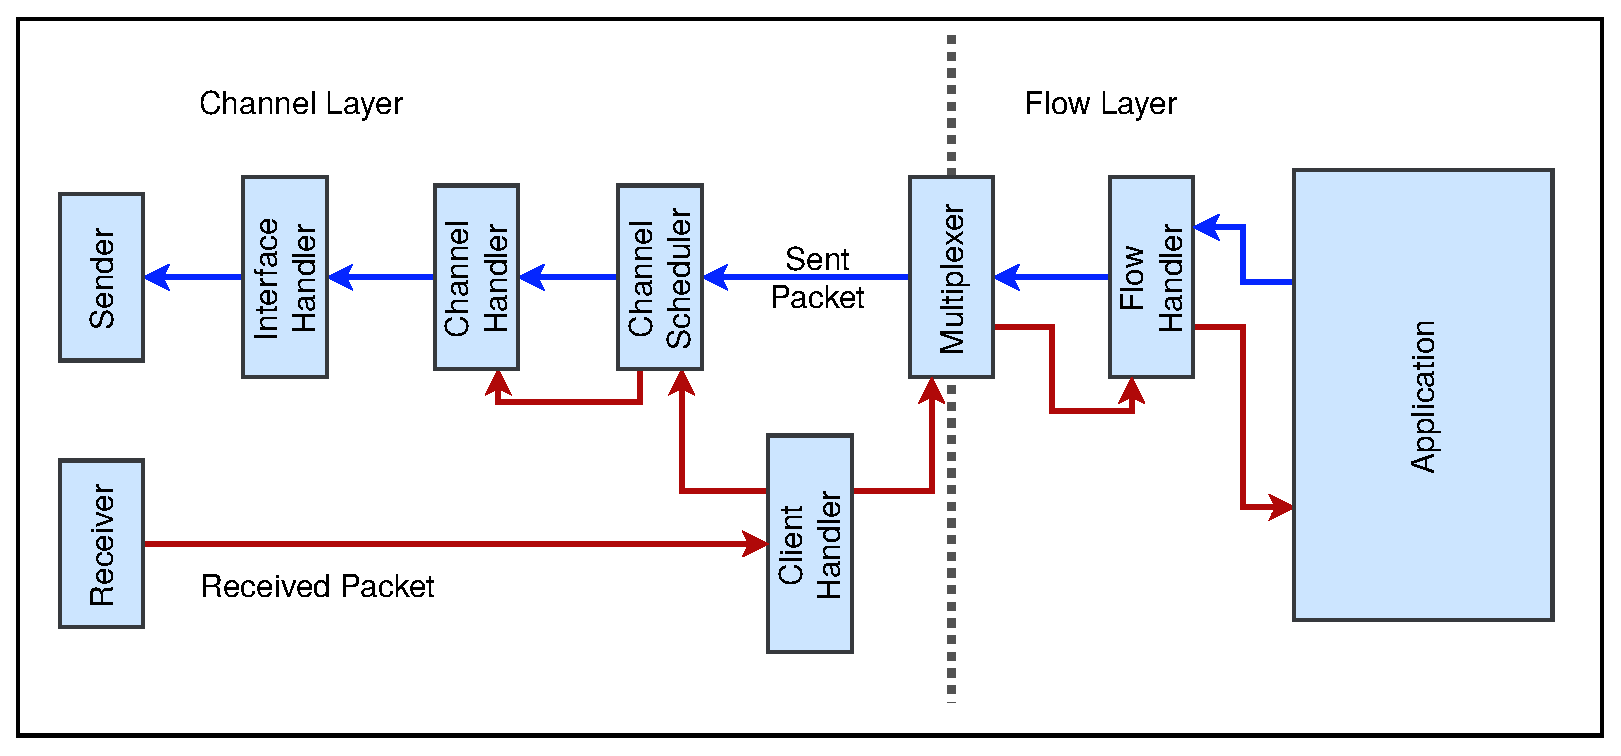
\includegraphics[width=.8\linewidth]{img/ModularDiagram}
    \caption{Internal Packet and Data Flow Diagram for Viscous}
    \label{fig:ModularDiagram}
\end{figure}

The various modules and their functionalities in Viscous are as follows. 

\subsubsection{Application}
An application is the users' application using the Viscous library. Viscous exposes few application programming interfaces (APIs) like (a) start the client, (b) add new flow, (c)send data, (d) stop/finish flow, and (e) stop client. These are the methods developed under Viscous, and an application needs to access the Viscous library to call the corresponding API from Viscous Application module. Few of these APIs are provided via callbacks, such as -- (a) addition of new clients, (b) reception of a new flow, (c) data received, and (d) flow closed. We use callback based APIs because it is easier to implement and it is expected that the callback methods are brief in general. This provides application programmability support with better performance guarantee in terms of execution time. 


\subsubsection{Flow Handler}
In Viscous, an application directly sends data to this module and receives from it. Flow handler packetizes the raw data from the application and sends packets to the lower layer for further processing. It does not need to store any outgoing packets, as the channel layer ensures the reliability. It only keeps track of the packets that it sends, to control the flow rate. Viscous uses a sliding window based flow control mechanism based on the receiver advertised window size. 

The flow handler also reorders the out of order packets that  it receives from the lower layer. There is a receive buffer that stores all the out of order packets. This buffer is an array of packets. The first index of this packet array point to the next expected packet sequence. Whenever the flow handler receives one or more contiguous packets from the expected sequence, it delivers the data from those flows to the application. In Viscous, there is one independent flow handler instance for each of the flows.

\subsubsection{Multiplexer}
The multiplexer is responsible for multiplexing the outgoing packets from multiple flows and forwards them to the packet scheduler. It is also responsible for demultiplexing incoming packets and forwarding them to the appropriate flow handler. In the event of an unknown flow ID in the incoming packet, it simply creates a new flow handler for the new packet. Validation of the packet is done mainly by the channel handler.

\subsubsection{Client Handler}
The client handler is the manager of Viscous protocol API. All incoming packets go through this module. For incoming packets, it checks the packet's validity using the fingerprint.  After validation, it forwards each incoming packet to the channel handler via channel scheduler for further validation and processing of the congestion control algorithm. If the channel handler returns a packet with marking as a valid packet, it forwards the packet to the multiplexer.

\subsubsection{Channel Scheduler}
It schedules the channel for the outgoing packets. The channel scheduler schedules outgoing packets to one of the channels. As mentioned earlier, we have used ACK driven channel scheduler in Viscous design. A packet is scheduled to a channel only when the channel is capable of sending new packets i.e. after receiving the acknowledgment packet. %\noteam{We need to give some reference. Sourav can help.}

\subsubsection{Channel Handler}
Channel handler is responsible for reliable communication and congestion control in the network. Instead of trying to build new congestion control algorithm, we have followed the standard TCP~\cite{RFC2582} congestion control algorithm for the Viscous implementation version $1.0$. We mimic TCP New Reno algorithm as given in RFC2582~\cite{RFC2582} and other RFCs, such as~\cite{RFC2581,RFC2988,RFC2001,RFC0793} with some modifications. These modifications are as follows:
\begin{itemize}
    \item Channel handler handles packets, not the byte streams. So, the sequence number represents a packet, not a byte. 
    \item Each acknowledgment packet contains the original sequence number, that is the sequence number of the packet for which this acknowledgment is triggered. It gives a similar effect as TCP SACK~\cite{RFC2018}.
    \item We have modified the fast recovery phase described in RFC2581~\cite{RFC2582} with SACK modification. After receiving the first partial new acknowledgment, the channel handler sends all the unacknowledged (via SACK or the original ACK in the packet header) packets for each duplicate ACK. This modification reduces retransmission due to timeout events when a burst of packets get lost in the network.
\end{itemize}

\subsubsection{Receiver}
A Viscous receiver is an independent module run as an independent thread. Its only job is to wait for a datagram on a datagram socket (i.e. UDP socket). Whenever some UDP packets arrive at a Viscous receiver, it receives the packets and forwards them to the channel handler.

\subsubsection{Sender}
It is also an independent module. Only one instance of Viscous sender can be there for an application. The Viscous sender checks a common queue with channel handlers. Whenever some channel handler decides to send a packet, it put the packet in a common queue. Then the sender picks up the packet from the queue and sends to the network via packet socket interface. It can be noted that the standard Linux datagram socket does not allow to mention the interface ID for sending a packet, which is required for multi-interface packet transmission. Therefore we use the packet socket API to encapsulate a Viscous packet inside an UDP datagram followed by a MAC frame, and then send it to the network. Using the MAC frame, we can decide the interface through which the packet can be transmitted. This supports multi-homing over Viscous implementation.  
%
%We use packet socket interface for sending purpose. There is no way define sending network interface in datagram socket \acrshort{api}. So, we encode Mac frame, then send it to the network. This method allows us to send through any interface we want.

Although using packet-socket we can send a packet through any interface we want, however the Unix network policy does not permit us to do so at the user level. To overcome the restriction with Unix systems, we follow the routing configuration\footnote{http://multipath-tcp.org/pmwiki.php/Users/ConfigureRouting} given by MPTCP implementation. Next we discuss the performance improvement that we achieve for Viscous under various network scenarios, compared to TCP Cubic, QUIC and MPTCP. 

%\subsection{Mobility}
%\noteam{write it down}
    \section{Experimental Evaluation}

To evaluate the performance of Viscous, we perform several experiments over \texttt{Mininet} network emulation platform. We have used two different network topologies for emulation, as shown in Fig.~\ref{fig:experimentalTopology1} (Topology-1) and Fig.~\ref{fig:experimentalTopology2} (Topology-2). In Topology-1, $H1$ has multiple interfaces, but $H2$ has a single interface; whereas in Topology-2, both $H1$ and $H2$ have multiple interfaces. In these two topologies, $H1$ and $H2$ act as the Viscous server and the Viscous client, respectively, or vice-versa. Rest of the hosts generate background traffic; and we evaluate the performance of Viscous both in the presence as well as in the absence of background traffic.  We compare the performance of Viscous with following protocols;
\begin{enumerate}
	\item[(i)] TCP: We have used TCP Cubic with the optimizations proposed in~\cite{largecwnd}, where as initial congestion window size of $10$ is used to avoid network underutilization for short-lived flows. 
	\item[(ii)] MPTCP: We have used Linux MPTCP kernel version 0.91 for our implementation.
	\item [(iii)] QUIC: We have compared Viscous with QUIC implementation provided by \texttt{libquic}\footnote{\url{https://github.com/devsisters/libquic} (last accessed: April 25, 2017)}. 
\end{enumerate}

\begin{figure}[!ht]
	\centering
	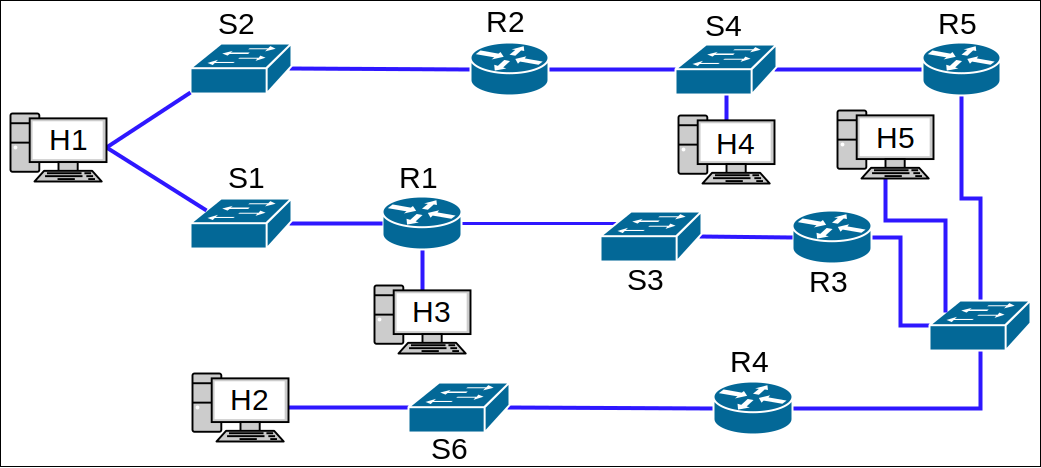
\includegraphics[width=0.7\linewidth]{img/experimentalTopology1}
	\caption{Topology 1: One of the end hosts has a single interface}
	\label{fig:experimentalTopology1}
\end{figure}

\begin{figure}[!ht]
	\centering
	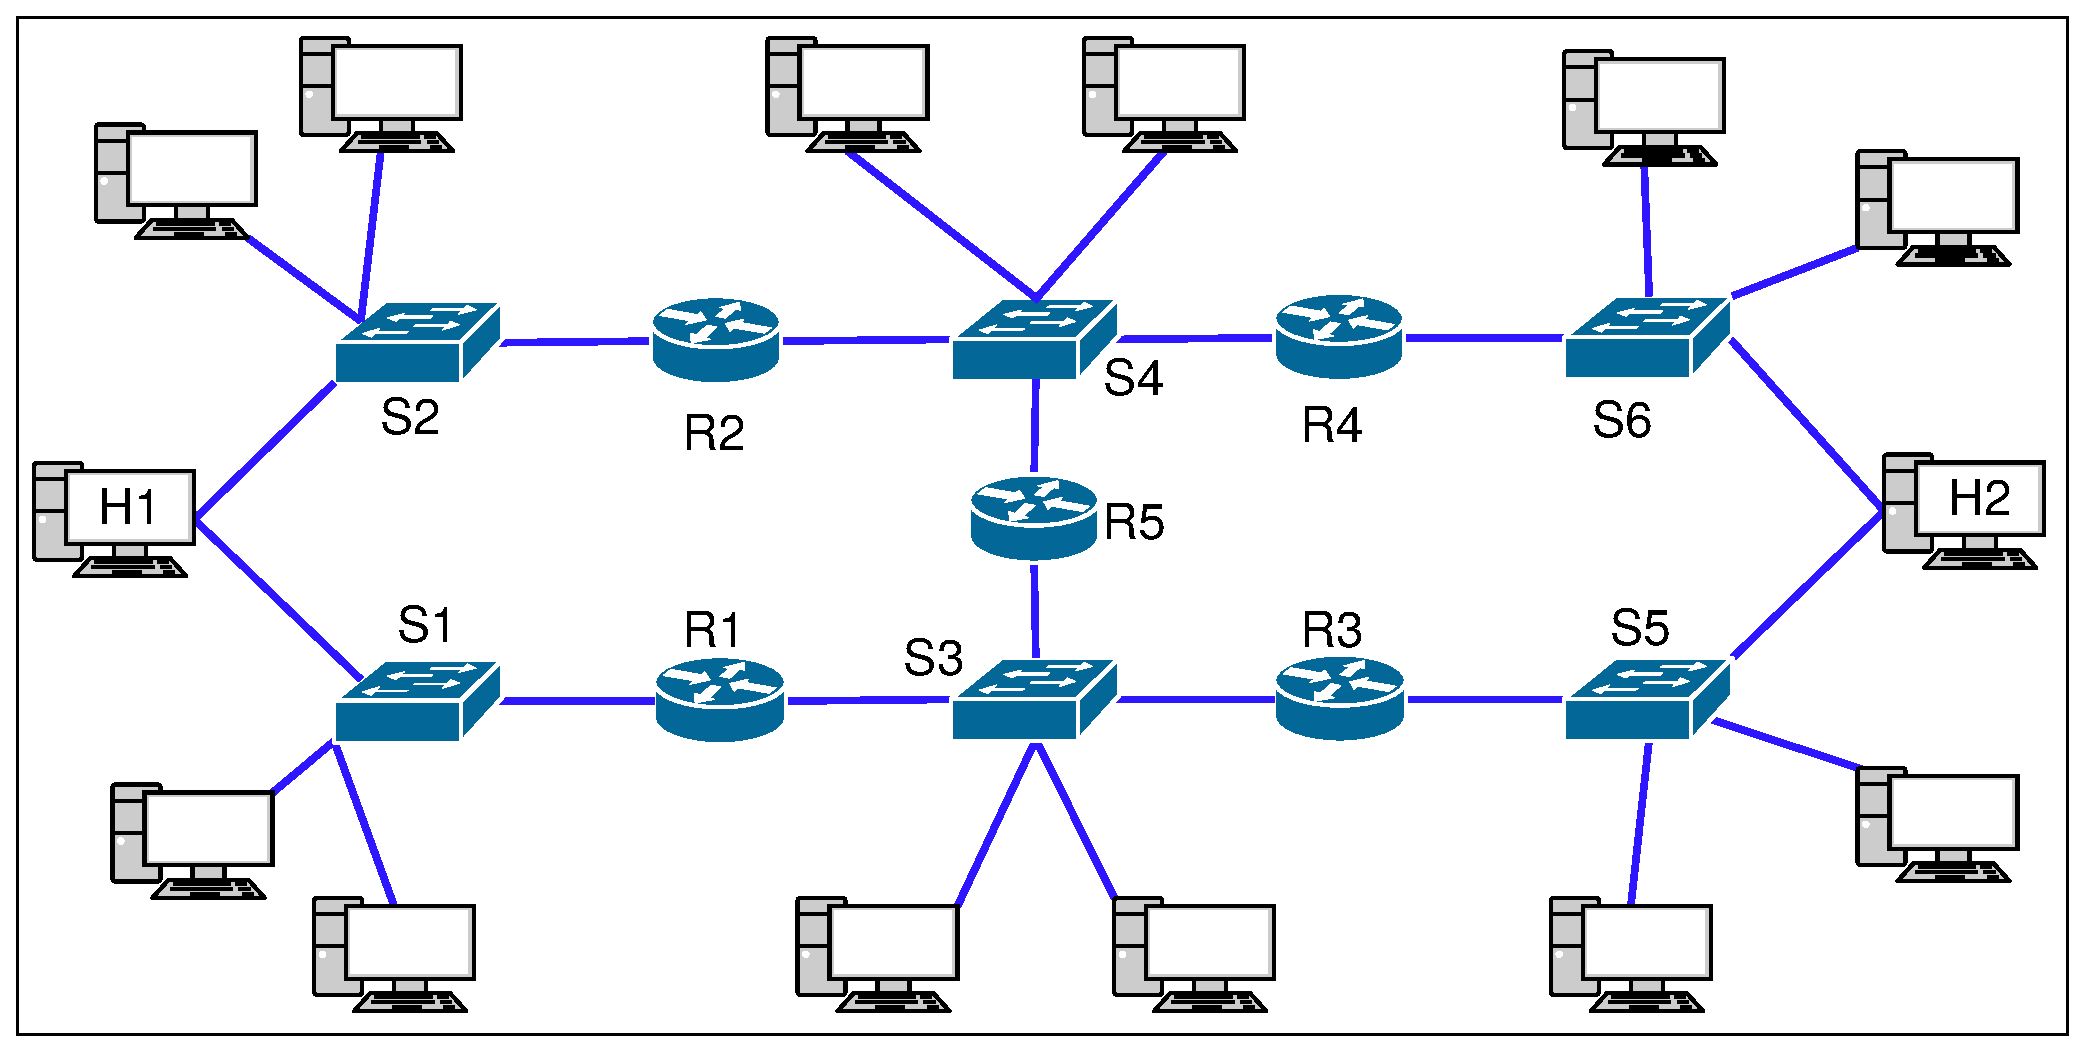
\includegraphics[width=0.7\linewidth]{img/experimentalTopology2}
	\caption{Topology 2: Both the end hosts have two interfaces}
	\label{fig:experimentalTopology2}
\end{figure}



\subsection{Experimental Setup}
The various hardware and operating system level parameters used in our experimental setup are as follows. 
\begin{itemize}
    \item \textbf{System configurations}: We have used Oracle VitualBox to create virtual machines which have been configured with \texttt{Mininet} kernel to support network interface virtualization. The guest machine configuration is as follows -- single core Intel i7-5500U 64bit CPU with clock speed of 2.40 GHz, RAM: 8GB. The host machine configuration is as follows -- Intel Genuin i7-5500U 64bit CPU with clock speed of 2.40GHz, RAM: 8GB with 250GB Solid State Drive.
    \item \textbf{Mininet}: Version 2.2.2 of \texttt{Mininet} kernel have been used to develop our test setup.
    \item \textbf{Kernel}: We have used the Linux kernel version 4.1.38.mptcp, which is patched with the MPTCP implementation.
    \item \textbf{MPTCP}: We have used MultiPath TCP version 0.91 for comparing the performance of Viscous with MPTCP.
    \item \textbf{Operating System}: In our virtual machine configurations for test setup, the guest operating system is Ubuntu 14.04.4 LTS, whereas the host operating system is Ubuntu 16.04.1 LTS. 
\end{itemize}
We setup the link bandwidths for different paths in the topologies as follows. In Topology-1, the two paths from the two interfaces of the host $H1$ up to the common point has a bandwidth of $50$ Mbps, and from the common point to the interface of the host $H2$ has a bandwidth of $100$ Mbps. For Topology-2, all the links have a link bandwidth of $100$ Mbps. 
 
Next we present the results and observations from various test scenarios as performed over the two topologies. 

\subsection{Experiment 1 (Performance over Topology-1 without any Background Traffic)}
\label{sub:experiment1}
In this experiment, we have explored the performance of \acrshort{quic}, \acrshort{tcp}, \acrshort{mptcp} and Viscous for a large numbers of short-lived flows, when there are no background flows. Therefore, the congestion in the network is generated by a single type of flow. This experiment has been performed over Topology-1. In Topology-1, there are two paths between $H1$ and $H2$, however $H2$ has a single interface. Here, we vary the RTT of the two paths from $16$ms to $320$ms, and observe the performance of the four protocols for end-to-end data transport. For every RTT setup, we have sent flows using multiple parallel threads to generate multiple simultaneous flows. For each thread, we have generated $100$ back-to-back flows; and have varied the flow duration based on an exponential distribution with mean flow duration of $25$ seconds. The number of parallel threads those generate the simultaneous flows have been varied from $1$ to $20$.  
%
%Overall delays in each path are varied from 16ms to 320ms. For each delay level, we have sent flows using multiple threads. In each thread, we sent 100 back-to-back short-lived flows. Data sizes for each flow are in exponential distribution \noteam{I forgot the parameters. I will add it later}. We vary the number of threads from 1 to 20. We compared the time required to complete the flows in Fig.~\ref{fig:exp6_time}.

%\begin{figure}[!t]
%	\captionsetup[subfigure]{}
%	\begin{center}
%		\subfloat[\label{fig:exp6_time_16}RTT=16ms]{
%			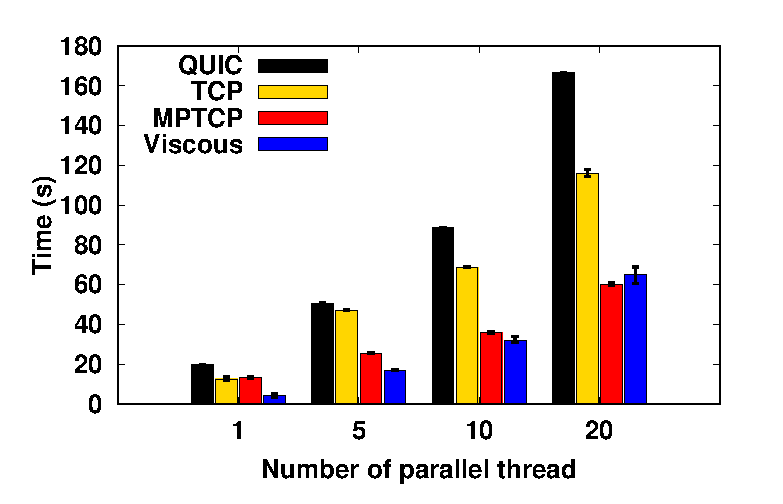
\includegraphics[width=0.24\linewidth]{img/exp6/time_elapsed_1}
%		}
%		\subfloat[\label{fig:exp6_time_80}RTT=80ms]{
%			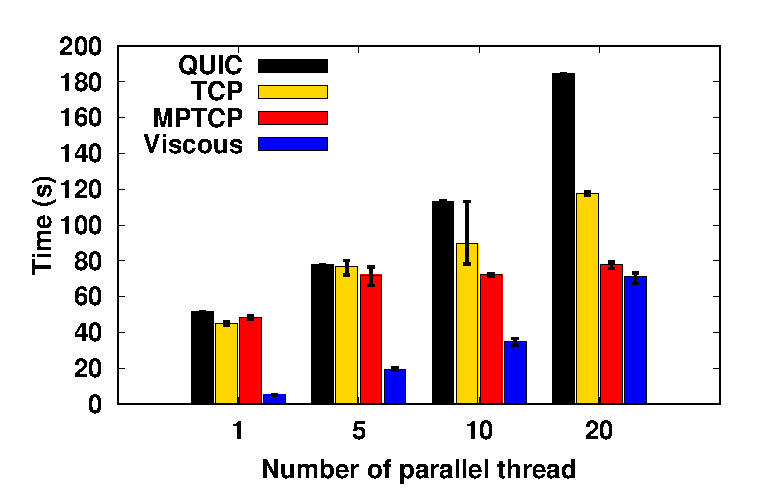
\includegraphics[width=0.24\linewidth]{img/exp6/time_elapsed_5}
%		}
%		\subfloat[\label{fig:exp6_time_160}RTT=160ms]{
%			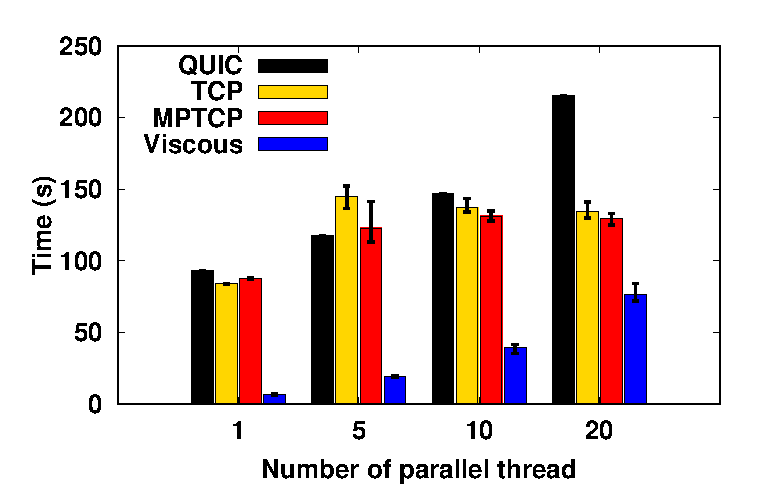
\includegraphics[width=0.24\linewidth]{img/exp6/time_elapsed_10}
%		}
%		\subfloat[\label{fig:exp6_time_320}RTT=320ms]{
%			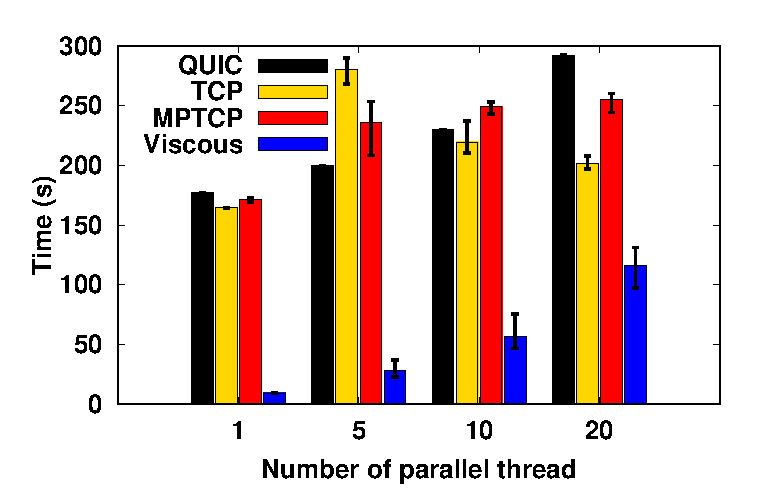
\includegraphics[width=0.24\linewidth]{img/exp6/time_elapsed_20}
%		}
%		\caption{\label{fig:exp6_time} Experiment 1: Flow Completion Time over Topology-1 without Background Flows}
%	\end{center}
%\end{figure}
\begin{figure}[!t]
    \begin{center}
        \begin{minipage}{0.45\linewidth}
            \centering
            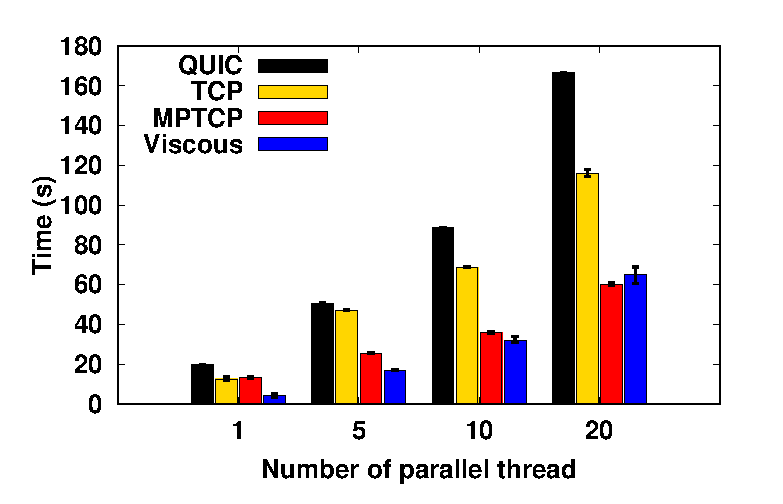
\includegraphics[width=\linewidth]{img/exp6/time_elapsed_1}
            \label{fig:exp6_time_16}
            \subcaption{RTT=16ms}
        \end{minipage}
        \begin{minipage}{0.45\linewidth}
            \centering
            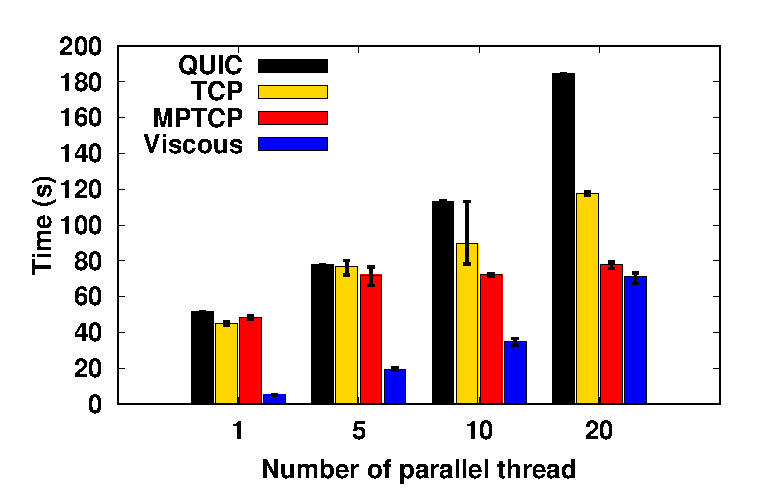
\includegraphics[width=\linewidth]{img/exp6/time_elapsed_5}
            \label{fig:exp6_time_80}
            \subcaption{RTT=80ms}
        \end{minipage}
        \begin{minipage}{0.45\linewidth}
            \centering
            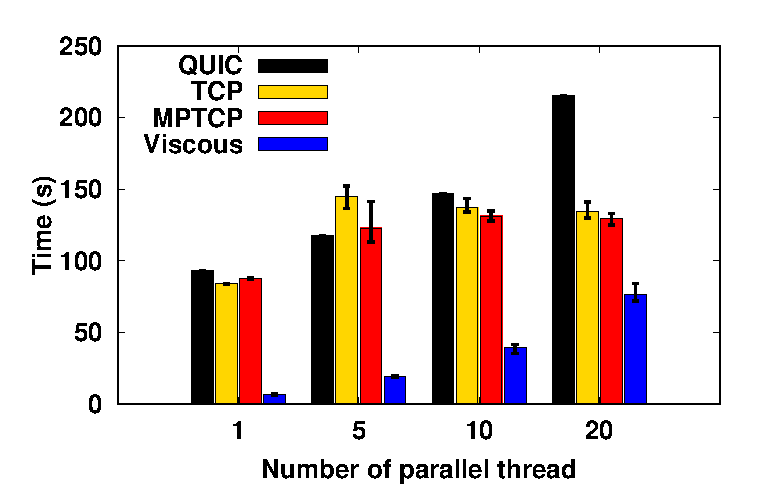
\includegraphics[width=\linewidth]{img/exp6/time_elapsed_10}
            \label{fig:exp6_time_160}
            \subcaption{RTT=160ms}
        \end{minipage}
        \begin{minipage}{0.45\linewidth}
            \centering
            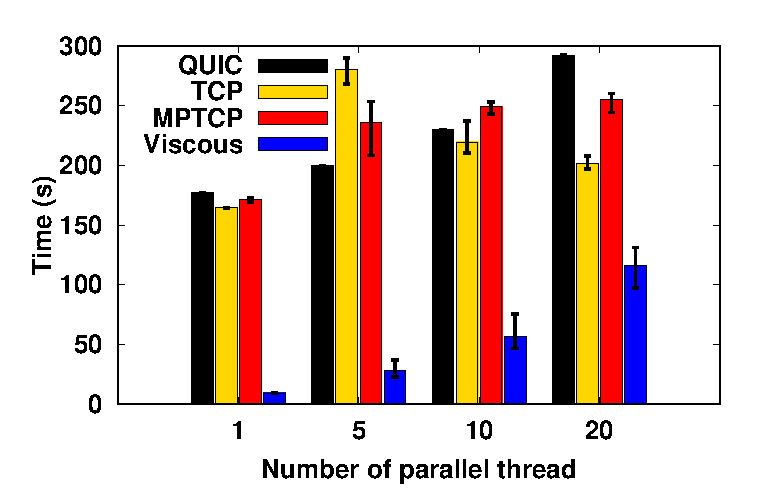
\includegraphics[width=\linewidth]{img/exp6/time_elapsed_20}
            \label{fig:exp6_time_320}
            \subcaption{RTT=320ms}
        \end{minipage}
        \caption{\label{fig:exp6_time}Experiment 1: Flow Completion Time over Topology-1 without Background Flows}
    \end{center}
\end{figure}

\begin{figure}[!t]
	\centering
	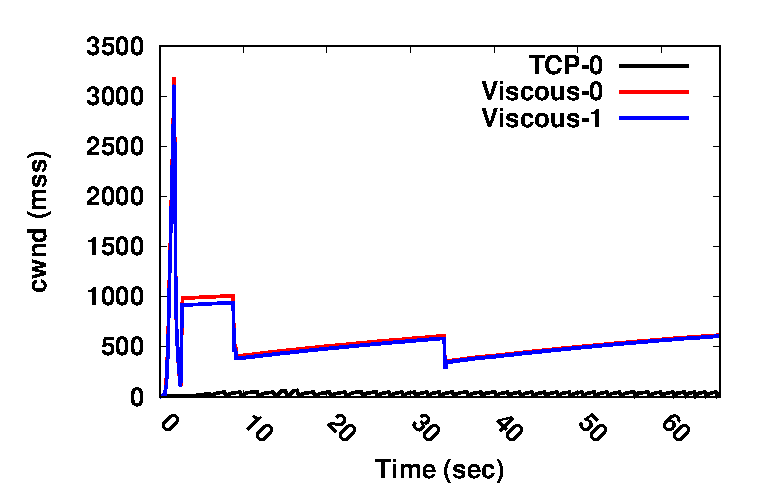
\includegraphics[width=0.5\linewidth]{img/exp6/cwnd_sample1_5_20}
	\caption{Experiment 1: Congestion Window Evolution}
	\label{fig:exp6_cwnd}
\end{figure}

First, we observe the average flow completion time for all the flows over Topology-1 without any background traffic, as shown in Fig.~\ref{fig:exp6_time}. From the figure, we can see that Viscous performs much better when multiple short-lived flows are transferred over the network. QUIC in this scenario does not perform good. Although QUIC can multiplex multiple flows coming from the application layer, it maintains flow specific congestion window, resulting in a slow start problem for the flows. Further, QUIC fails to utilize multiple interfaces available in the network which is one of the main reasons behind its poor performance over the test topology. MPTCP suffers from the path imbalance problem as discussed earlier, and TCP Cubic can not utilize multi-homing capacity for the flows. To analyze the effect of short-lived flows, we compare the congestion window evolution for TCP and Viscous for a specific case, as given in Fig.~\ref{fig:exp6_cwnd}, when RTT=$16$ ms and number of parallel thread = $5$. We observe that the average congestion window for TCP is significantly less. The congestion window evolutions for Viscous along the two paths have been shown (Viscous-0 and Viscous-1), and in both the paths, Viscous can achieve a significant higher values of the congestion window. Consequently, Viscous sub-flows can utilize the available bandwidth at the paths in a significantly better way for multiplexed short-lived flows. 

%
%
%it is clear that Viscous performs much better for multiple short flows. \acrshort{quic} is worse than everyone else. Even normal \acrshort{tcp} connection. We could not be able to collect any other information from \acrshort{quic}. For lower delay and a larger number of threads, \acrshort{mptcp} may have performed slightly better than Viscous (Thread 20 at Fig.~\ref{fig:exp6_time_16}). \acrshort{tcp} and \acrshort{mptcp} is suffering because it needs to setup connection for each flow and starts congestion window ($cwnd$) size from initial congestion window (which is ten mss for this setup). In Fig.~\ref{fig:exp6_cwnd}, we plot $cwnd$ evolution of \acrshort{tcp} and Viscous. Here we can see that for Viscous $cwnd$ grows normally. It crosses the slow-start phase and continues in congestion avoidance phase. However, for \acrshort{tcp} it is hardly visible.

%\begin{figure*}[!t]
%	\captionsetup[subfigure]{}
%	\begin{center}
%		\subfloat[\label{fig:exp6_goodput_16}RTT=16ms]{
%			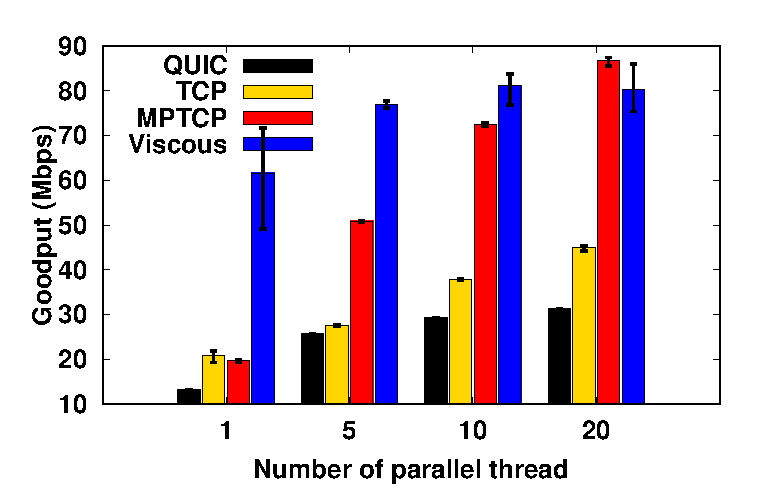
\includegraphics[width=0.24\linewidth]{img/exp6/goodput_1}
%		}
%		\subfloat[\label{fig:exp6_goodput_80}RTT=80ms]{
%			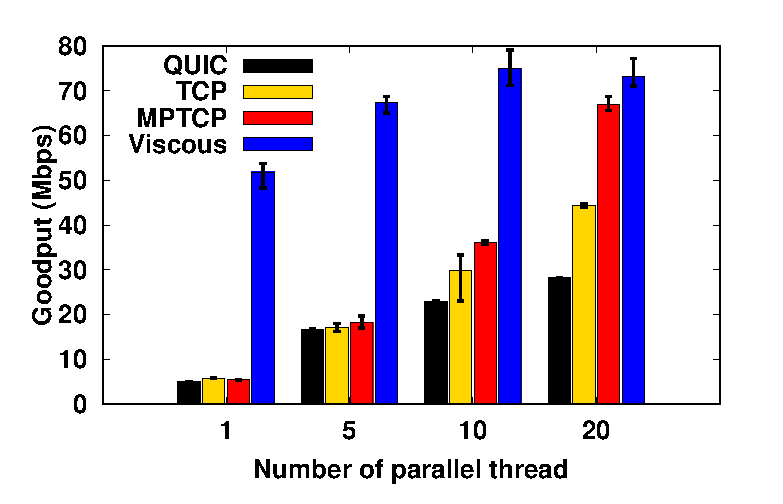
\includegraphics[width=0.24\linewidth]{img/exp6/goodput_5}
%		}
%		\subfloat[\label{fig:exp6_goodput_160}RTT=160ms]{
%			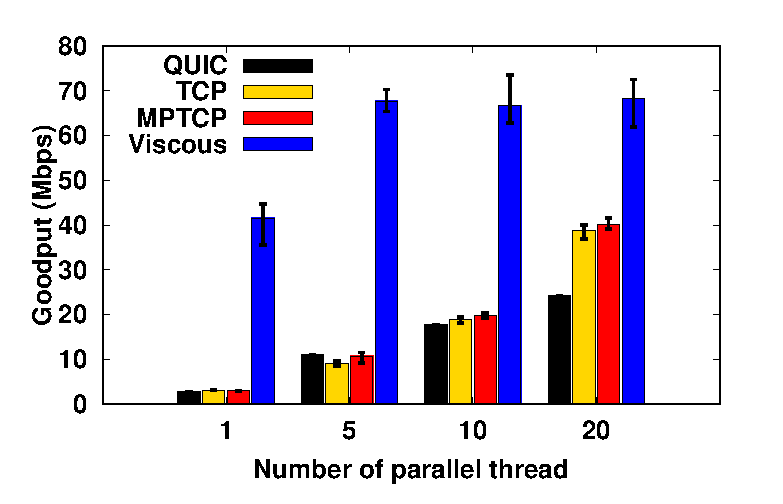
\includegraphics[width=0.24\linewidth]{img/exp6/goodput_10}
%		}
%		\subfloat[\label{fig:exp6_goodput_320}RTT=320ms]{
%			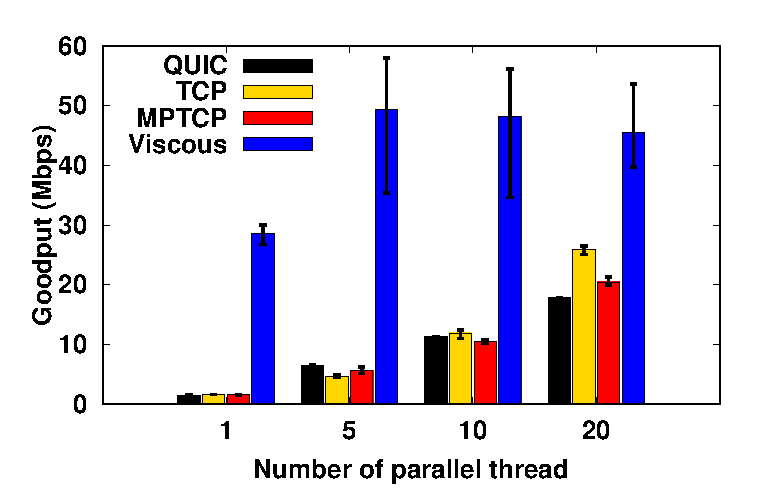
\includegraphics[width=0.24\linewidth]{img/exp6/goodput_20}
%		}
%		\caption{\label{fig:exp6_goodput}Experiment 1: Goodput over Topology-1 without Background Flows}
%	\end{center}
%\end{figure*}

\begin{figure}[!t]
    \begin{center}
        \begin{minipage}{0.45\linewidth}
            \centering
            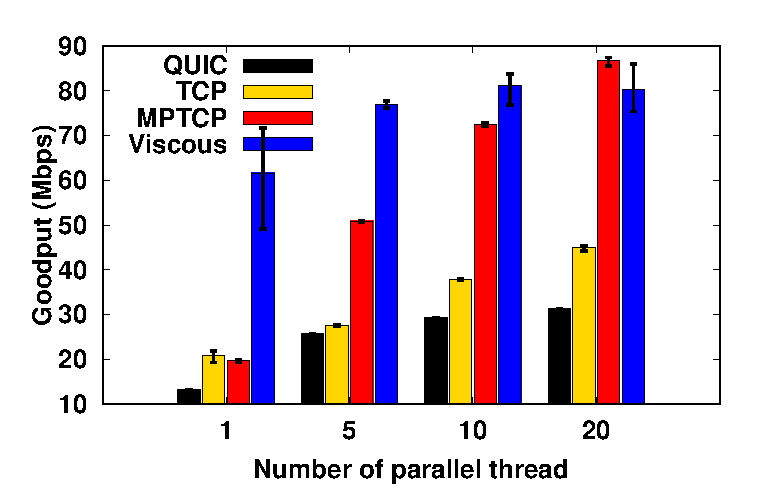
\includegraphics[width=\linewidth]{img/exp6/goodput_1}
            \label{fig:exp6_goodput_16}
            \subcaption{RTT=16ms}
        \end{minipage}
        \begin{minipage}{0.45\linewidth}
            \centering
            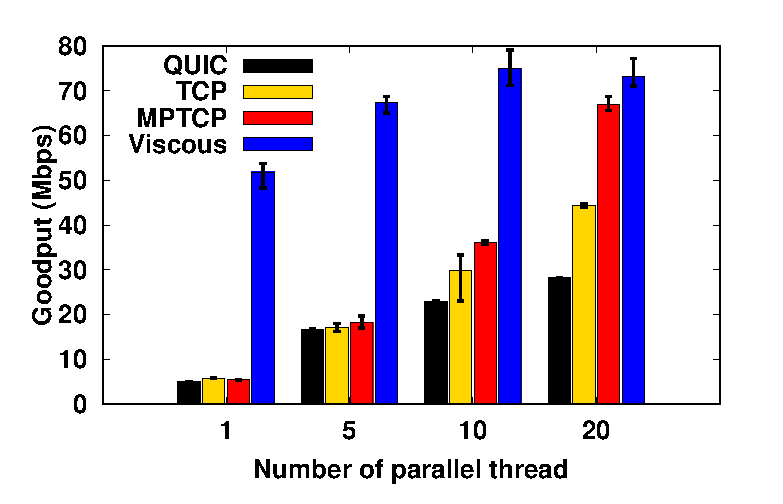
\includegraphics[width=\linewidth]{img/exp6/goodput_5}
            \label{fig:exp6_goodput_80}
            \subcaption{RTT=80ms}
        \end{minipage}
        \begin{minipage}{0.45\linewidth}
            \centering
            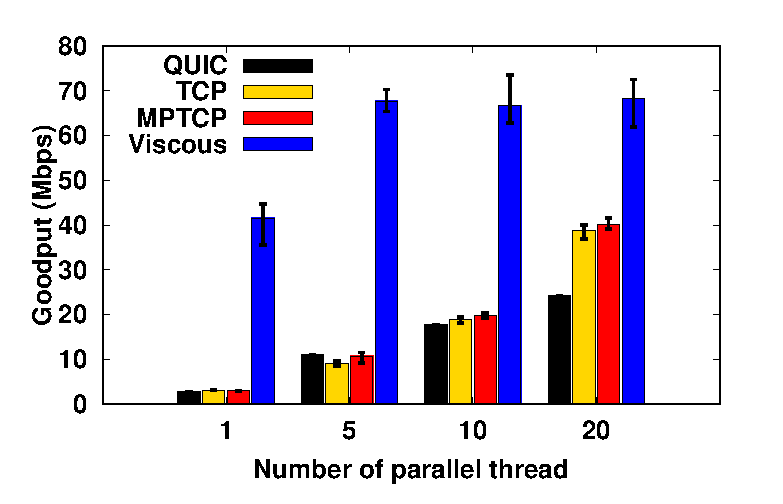
\includegraphics[width=\linewidth]{img/exp6/goodput_10}
            \label{fig:exp6_goodput_160}
            \subcaption{RTT=160ms}
        \end{minipage}
        \begin{minipage}{0.45\linewidth}
            \centering
            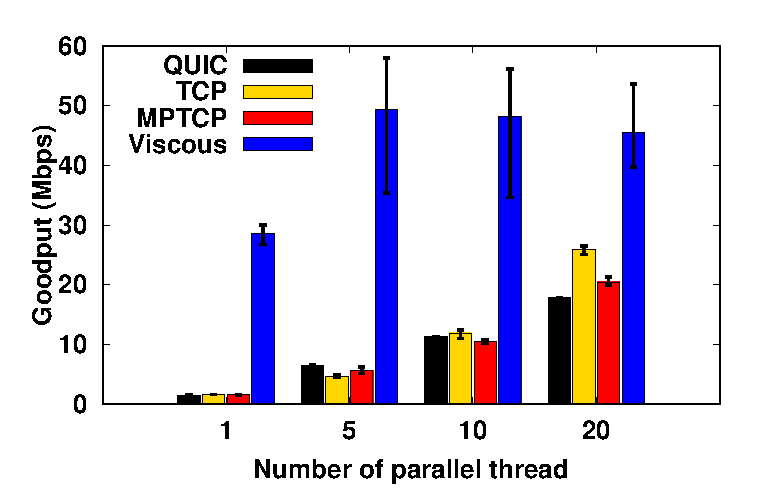
\includegraphics[width=\linewidth]{img/exp6/goodput_20}
            \label{fig:exp6_goodput_320}
            \subcaption{RTT=320ms}
        \end{minipage}
        \caption{\label{fig:exp6_goodput}Experiment 1: Goodput over Topology-1 without Background Flows}
    \end{center}
\end{figure}

Next, we observe the average goodput of the flows for the four different protocols under the same scenario, as shown in Fig.~\ref{fig:exp6_goodput}. Similar to the flow completion time, we observe that the goodput of Viscous is higher than all other protocols. Viscous can utilize the capacity of multiple paths through flow multiplexing and maintaining connection specific congestion window evolution over the time; and therefore it attains higher goodput compared to other competing end-to-end protocols. Further, we observe that the goodput for Viscous is significantly boosted up compared to other protocols, when RTT of the paths is high. This indicates that Viscous overshoots the performance compared to other protocols when network condition is poor. QUIC, TCP and MPTCP can not cope up with the poor network condition, whereas Viscous can effectively utilize the available capacity under all the scenarios. The reason behind this better performance is the Viscous channel scheduler, that uses a self-clocking mechanism to schedule and trigger the transmissions over multiple channels based on the ACK packets. This self-clocking helps in proper utilization of the channels even under poor RTT conditions. 


\subsection{Experiment 2 (Performance over Topology-1 in the Presence of Background Flows)}

\begin{figure}[!t]
	\begin{center}
		\begin{minipage}{0.45\linewidth}
			\centering
			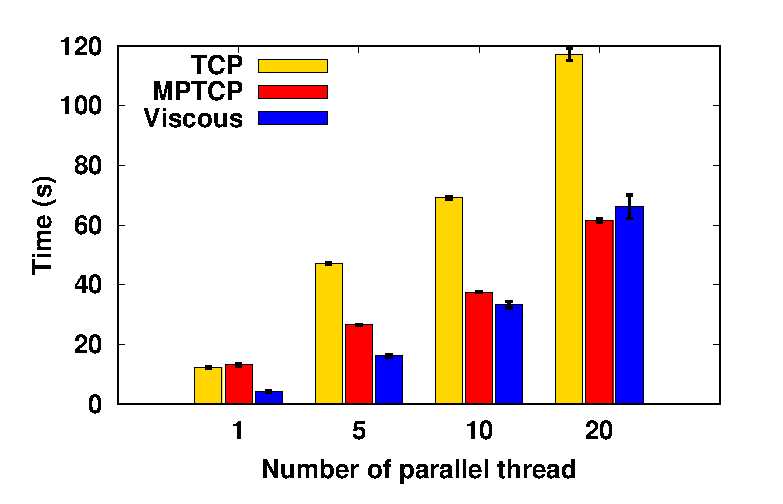
\includegraphics[width=\linewidth]{img/exp7/time_elapsed_1}
			\label{fig:exp7_time_16}
			\subcaption{RTT=16ms}
		\end{minipage}
		\begin{minipage}{0.45\linewidth}
			\centering
			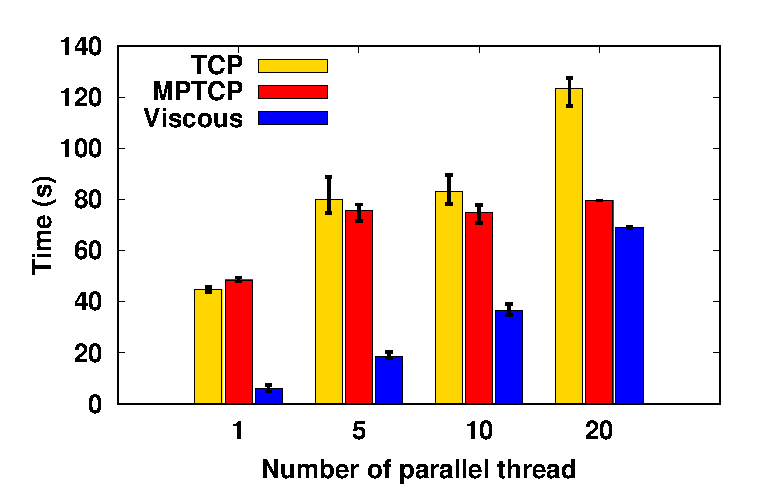
\includegraphics[width=\linewidth]{img/exp7/time_elapsed_5}
			\label{fig:exp7_time_80}
			\subcaption{RTT=80ms}
		\end{minipage}
		\begin{minipage}{0.45\linewidth}
			\centering
			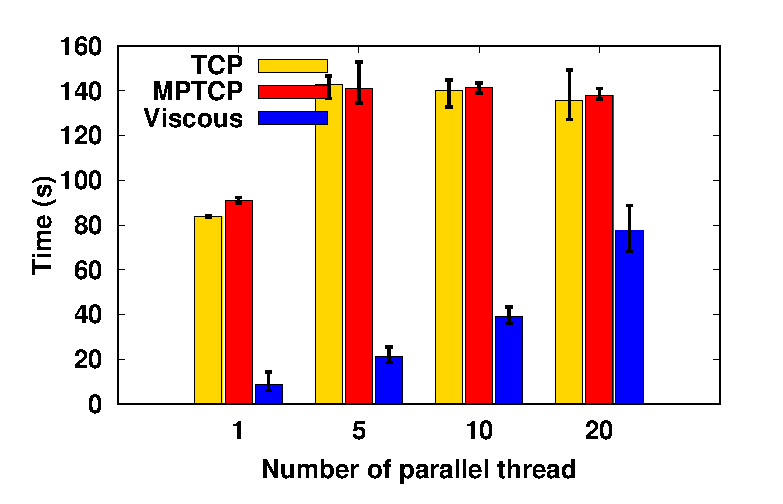
\includegraphics[width=\linewidth]{img/exp7/time_elapsed_10}
			\label{fig:exp7_time_160}
			\subcaption{RTT=160ms}
		\end{minipage}
		\begin{minipage}{0.45\linewidth}
			\centering
			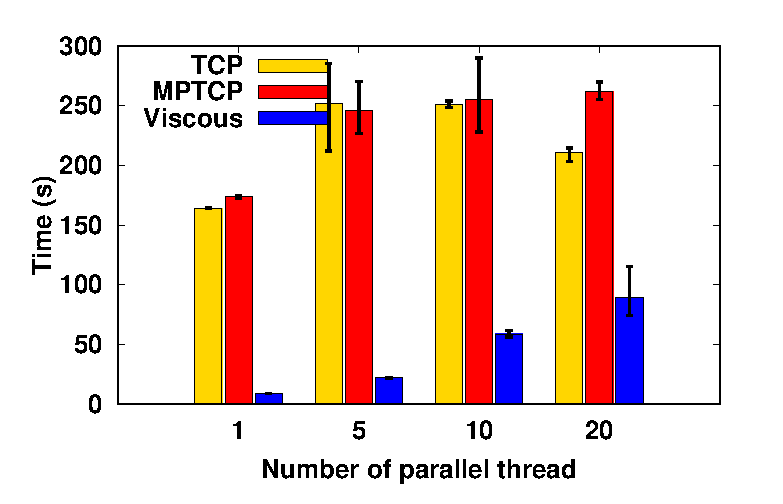
\includegraphics[width=\linewidth]{img/exp7/time_elapsed_20}
			\label{fig:exp7_time_320}
			\subcaption{RTT=320ms}
		\end{minipage}
		\caption{\label{fig:exp7_time}Experiment 2: Flow Completion Time over Topology-1 with Background Traffic}
	\end{center}
\end{figure}

\begin{figure}[!t]
	\centering
	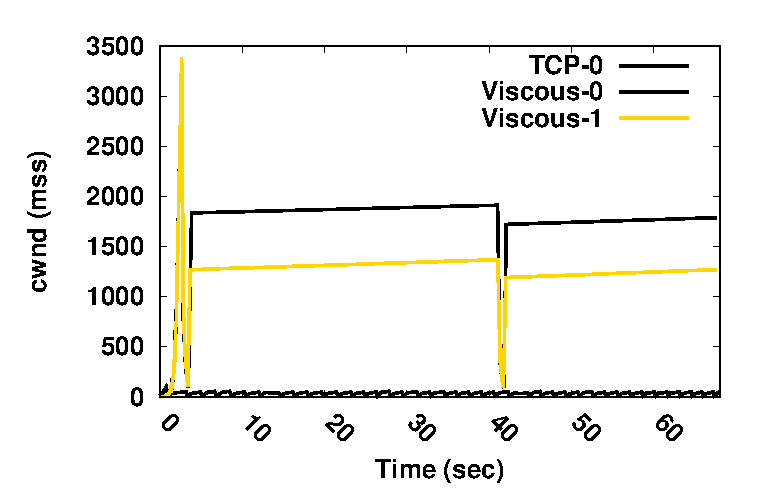
\includegraphics[width=0.5\linewidth]{img/exp7/cwnd_sample2_10_20}
	\caption{Experiment 2: Congestion window evolution}
	\label{fig:exp7_cwnd}
\end{figure}


\begin{figure}[!t]
	\begin{center}
		\begin{minipage}{0.45\linewidth}
			\centering
			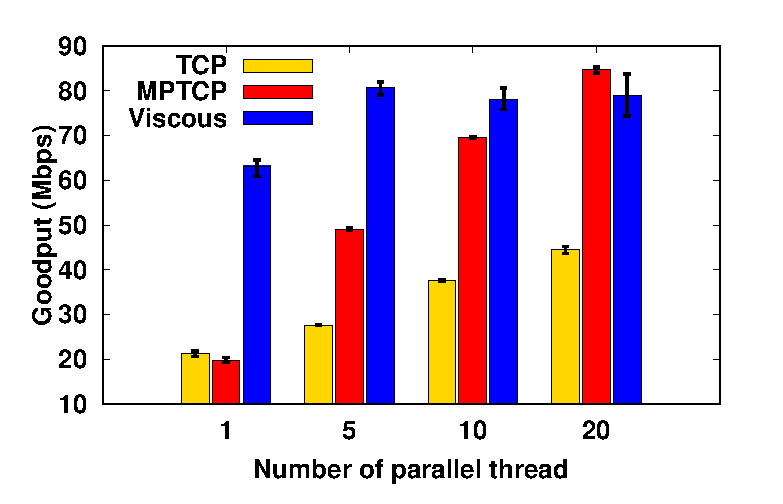
\includegraphics[width=\linewidth]{img/exp7/goodput_1}
			\label{fig:exp7_goodput_16}
			\subcaption{RTT=16ms}
		\end{minipage}
		\begin{minipage}{0.45\linewidth}
			\centering
			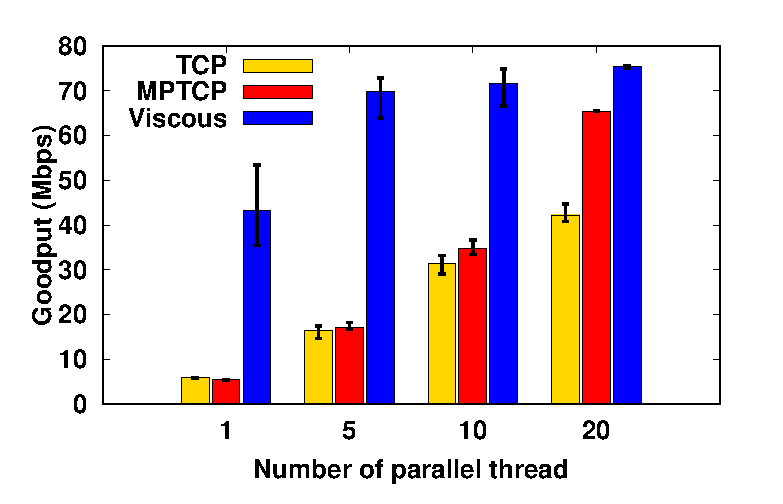
\includegraphics[width=\linewidth]{img/exp7/goodput_5}
			\label{fig:exp7_goodput_80}
			\subcaption{RTT=80ms}
		\end{minipage}
		\begin{minipage}{0.45\linewidth}
			\centering
			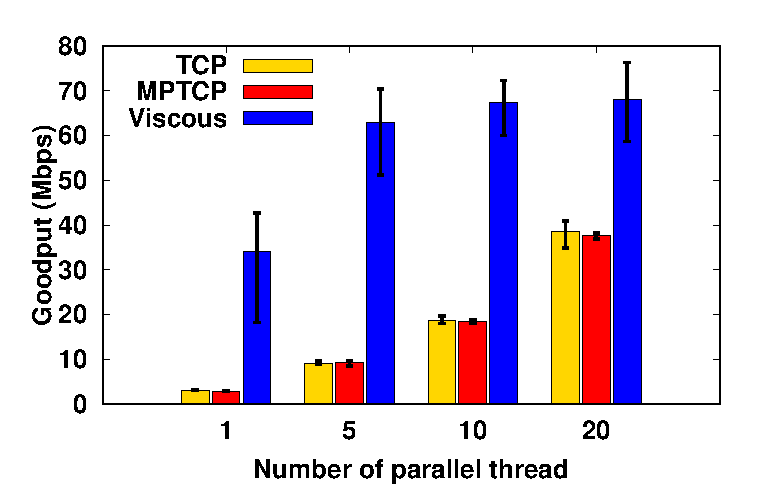
\includegraphics[width=\linewidth]{img/exp7/goodput_10}
			\label{fig:exp7_goodput_160}
			\subcaption{RTT=160ms}
		\end{minipage}
		\begin{minipage}{0.45\linewidth}
			\centering
			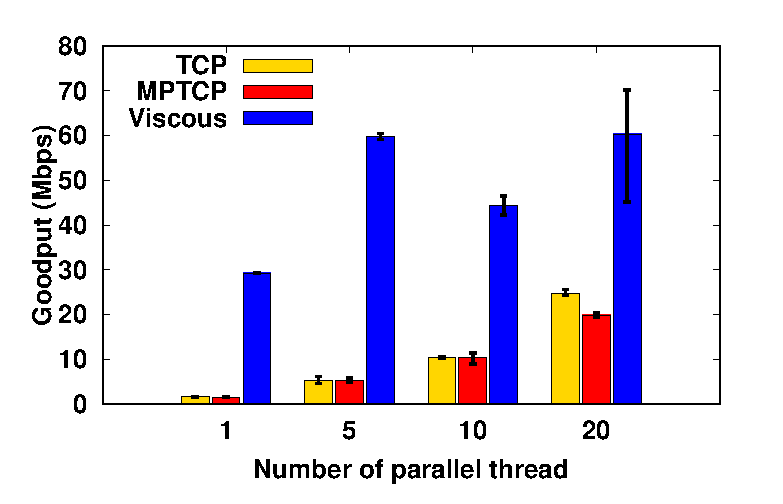
\includegraphics[width=\linewidth]{img/exp7/goodput_20}
			\label{fig:exp7_goodput_320}
			\subcaption{RTT=320ms}
		\end{minipage}
		\caption{\label{fig:exp7_goodput}Experiment 2: Goodput over Topology-1 with Background Traffic}
	\end{center}
\end{figure}



We have performed the similar experiment as given in Experiment 1, however, in this scenario we have considered the performance of the protocols in the presence of  background traffic. To generate background traffic, we have sent continuous HTTP traffic from $H3$ to $H4$ and $H5$ over Topology-1. This traffic is also in the form of the exponential in nature with mean number of packets as $25$ per second. We have plotted the results in Fig.~\ref{fig:exp7_time}, Fig.~\ref{fig:exp7_goodput} and Fig.~\ref{fig:exp7_cwnd}, for average flow completion time, average goodput for the flows and congestion window evolution over time, respectively. Similar to the previous case, we have found that Viscous performs much better than other competing protocols even in the presence of background traffic. Viscous takes less time than other end-to-end protocols, and the drop in performance for Viscous is comparatively less than other protocols when background traffic is present. The effectiveness of Viscous lies in the fact of proper utilization of available capacity over multiple paths, even in the presence of short-lived flows. Fig.~\ref{fig:exp7_cwnd} shows that Viscous can attain a significant boost in congestion window size at both the paths, compared to TCP Cubic. 

%\begin{figure*}[!t]
%    \captionsetup[subfigure]{}
%    \begin{center}
%        \subfloat[\label{fig:exp7_time_16}RTT=16ms]{
%            \includegraphics[width=0.24\linewidth]{img/exp7/time_elapsed_1}
%        }
%        \subfloat[\label{fig:exp7_time_80}RTT=80ms]{
%            \includegraphics[width=0.24\linewidth]{img/exp7/time_elapsed_5}
%        }
%        \subfloat[\label{fig:exp7_time_160}RTT=160ms]{
%            \includegraphics[width=0.24\linewidth]{img/exp7/time_elapsed_10}
%        }
%        \subfloat[\label{fig:exp7_time_320}RTT=320ms]{
%            \includegraphics[width=0.24\linewidth]{img/exp7/time_elapsed_20}
%        }
%        \caption{\label{fig:exp7_time}Experiment 2: Flow Completion Time over Topology-1 with Background Traffic}
%    \end{center}
%\end{figure*}
%
%\begin{figure*}[!t]
%    \captionsetup[subfigure]{}
%    \begin{center}
%        \subfloat[\label{fig:exp7_goodput_16}RTT=16ms]{
%            \includegraphics[width=0.24\linewidth]{img/exp7/goodput_1}
%        }
%        \subfloat[\label{fig:exp7_goodput_80}RTT=80ms]{
%            \includegraphics[width=0.24\linewidth]{img/exp7/goodput_5}
%        }
%        \subfloat[\label{fig:exp7_goodput_160}RTT=160ms]{
%            \includegraphics[width=0.24\linewidth]{img/exp7/goodput_10}
%        }
%        \subfloat[\label{fig:exp7_goodput_320}RTT=320ms]{
%            \includegraphics[width=0.24\linewidth]{img/exp7/goodput_20}
%        }
%        \caption{\label{fig:exp7_goodput}Experiment 2: Goodput over Topology-1 with Background Traffic}
%    \end{center}
%\end{figure*}


\subsection{Experiment 3 (Performance over Topology-2 in the Presence of Background Flows)}

%\begin{figure*}[!t]
%	\captionsetup[subfigure]{}
%	\begin{center}
%		\subfloat[\label{fig:exp10_time_16}RTT=16ms]{
%			\includegraphics[width=0.24\linewidth]{img/exp10/time_elapsed_1}
%		}
%		\subfloat[\label{fig:exp10_time_80}RTT=80ms]{
%			\includegraphics[width=0.24\linewidth]{img/exp10/time_elapsed_5}
%		}
%		\subfloat[\label{fig:exp10_time_160}RTT=160ms]{
%			\includegraphics[width=0.24\linewidth]{img/exp10/time_elapsed_10}
%		}
%		\subfloat[\label{fig:exp10_time_320}RTT=320ms]{
%			\includegraphics[width=0.24\linewidth]{img/exp10/time_elapsed_20}
%		}
%		\caption{\label{fig:exp10_time}Experiment 3: Flow Completion Time over Topology-2 without Background Traffic}
%	\end{center}
%\end{figure*}
%
%\begin{figure*}[!t]
%	\captionsetup[subfigure]{}
%	\begin{center}
%		\subfloat[\label{fig:exp10_goodput_16}RTT=16ms]{
%			\includegraphics[width=0.24\linewidth]{img/exp10/goodput_1}
%		}
%		\subfloat[\label{fig:exp10_goodput_80}RTT=80ms]{
%			\includegraphics[width=0.24\linewidth]{img/exp10/goodput_5}
%		}
%		\subfloat[\label{fig:exp10_goodput_160}RTT=160ms]{
%			\includegraphics[width=0.24\linewidth]{img/exp10/goodput_10}
%		}
%		\subfloat[\label{fig:exp10_goodput_320}RTT=320ms]{
%			\includegraphics[width=0.24\linewidth]{img/exp10/goodput_20}
%		}
%		\caption{\label{fig:exp10_goodput}Experiment 3: Average Goodput over Topology-2 without Background Traffic}
%	\end{center}
%\end{figure*}

\begin{figure}[!t]
    \begin{center}
        \begin{minipage}{0.45\linewidth}
            \centering
            \includegraphics[width=\linewidth]{img/exp10/time_elapsed_1}
            \label{fig:exp10_time_16}
            \subcaption{RTT=16ms}
        \end{minipage}
        \begin{minipage}{0.45\linewidth}
            \centering
            \includegraphics[width=\linewidth]{img/exp10/time_elapsed_5}
            \label{fig:exp10_time_80}
            \subcaption{RTT=80ms}
        \end{minipage}
        \begin{minipage}{0.45\linewidth}
            \centering
            \includegraphics[width=\linewidth]{img/exp10/time_elapsed_10}
            \label{fig:exp10_time_160}
            \subcaption{RTT=160ms}
        \end{minipage}
        \begin{minipage}{0.45\linewidth}
            \centering
            \includegraphics[width=\linewidth]{img/exp10/time_elapsed_20}
            \label{fig:exp10_time_320}
            \subcaption{RTT=320ms}
        \end{minipage}
        \caption{\label{fig:exp10_time}Experiment 3: Flow Completion Time over Topology-2 without Background Traffic}
        \end{center}
    \end{figure}
    
    \begin{figure}[!t]
        \begin{center}
            \begin{minipage}{0.45\linewidth}
                \centering
                \includegraphics[width=\linewidth]{img/exp10/goodput_1}
                \label{fig:exp10_goodput_16}
                \subcaption{RTT=16ms}
            \end{minipage}
            \begin{minipage}{0.45\linewidth}
                \centering
                \includegraphics[width=\linewidth]{img/exp10/goodput_5}
                \label{fig:exp10_goodput_80}
                \subcaption{RTT=80ms}
            \end{minipage}
            \begin{minipage}{0.45\linewidth}
                \centering
                \includegraphics[width=\linewidth]{img/exp10/goodput_10}
                \label{fig:exp10_goodput_160}
                \subcaption{RTT=160ms}
            \end{minipage}
            \begin{minipage}{0.45\linewidth}
                \centering
                \includegraphics[width=\linewidth]{img/exp10/goodput_20}
                \label{fig:exp10_goodput_320}
                \subcaption{RTT=320ms}
            \end{minipage}
            \caption{\label{fig:exp10_goodput}Experiment 3: Average Goodput over Topology-2 without Background Traffic}
        \end{center}
    \end{figure}


Next we perform similar experiments over Topology-2, where both the server and the client have multiple interfaces. The results are shown in Fig.~\ref{fig:exp10_time} for average flow completion time, and in Fig.~\ref{fig:exp10_goodput} for average goodput of the flows. Similar to the earlier scenarios, here we observe that Viscous attains better goodput and lower flow completion time compared to QUIC, TCP Cubic and MPTCP. Similar to the previous case, QUIC in this scenario as well, does not perform good for short flows. Although QUIC can multiplex multiple flows coming from the application layer, it maintains flow specific congestion window, resulting in a slow start problem for the flows. Further, QUIC fails to utilize multiple interfaces available in the network which is one of the main reasons behind its poor performance over the test topology. MPTCP suffers from the path imbalance problem as discussed earlier, and TCP Cubic can not utilize multi-homing capacity for the flows. As a consequence, we observe significant performance improvement using Viscous, compared to other protocols. Additionally, we observe that in this scenario, Viscous attains better goodput compared to the goodput over Topology-1, as shown in Fig.~\ref{fig:exp6_goodput}. This indicates that Viscous can properly utilize multihoming of devices, both at the Viscous client as well as at the the Viscous server. 


\subsection{Experiment 4: Performance for Long Flows over a Single Path -- Worst Case Performance of Viscous}


\begin{figure}[!t]
	\centering
	\includegraphics[width=0.5\linewidth]{img/exp1/tcp-mpudp_res}
	\caption{Performance Comparison between Viscous and TCP for Long Flows over a Single Path}
	\label{fig:exp1_singlepath}
\end{figure}


Till now we have tested the performance of Viscous for short-lived flows. To compare its performance for long flows, we have performed this experiment, where we send various size of file from the host $H3$ to the host $H2$ over Topology-1. We plot the time required to transmit a complete file over the network using TCP and Viscous, when both uses only one path in the network. The results are plotted in Fig.~\ref{fig:exp1_singlepath}. From this figure, we observe that the performance of Viscous is almost equal for long flows over a single path, which we consider as the worst case performance for this protocol. This experiment shows that in the worst case, Viscous performs as good as TCP Cubic, however, under the scenarios with multiple short-lived event triggered or user generated flows, Viscous can significantly boost up the end-to-end performance. 



    \subsection{Summary}
In this section, we developed a systematic analysis of web based adaptive streaming performance over \ac{QUIC} and compared it with \ac{TCP} enabled video streaming. We developed a testbed to automatically download $175$ YouTube videos with different quality levels and of different sizes using both \ac{QUIC} enabled and \ac{TCP} enabled streaming. From thorough analysis, we observed that although \ac{QUIC} improves data download performance even at poor network condition, the benefits do not get directly translated to adaptive video streaming over the web, when \ac{QoE} metrics are considered. 

This section primarily analyzed the performance from the context of YouTube \ac{ABR} streaming. In the next section, we discuss about a more generalized analysis, where we consider various recent \ac{ABR} streaming algorithms. 
%	\input{Introduction.tex}
%	\section{Motivation}

Internet is the network which connects different computing devices all over the globe. The conceptual platform form Internet and all othe computer network are followed by Internet protocol suite which is commonly known as TCP/IP model. TCP/IP model is made of two original protocol \acrfull{tcp} and \acrfull{ip}. TCP/IP protocol suite first developed in 1975 and become standard for inter-networking.

Internet become more popular with \acrfull{www}, which server content as html page to user over the application layer proto \acrfull{http}. \acrshort{www} started with serving small text based pages. Now, it serves web based application which are complement of Desktop application. With the help of \acrshort{www}, Internet grows to many folds. Recent studies show that, most of the Internet traffic served by \acrshort{http} alone. Even in the boom of Smart-Phone, most of the application communicate with their server using \acrshort{http} only.

\acrshort{http} uses \acrshort{tcp} as underlying transport layer. \acrshort{tcp} provides application to application to connection oriented reliable data communication. Although \acrshort{tcp} serves the purpose of \acrshort{http} and other application layer protocol, it have some inherent problem. They are:
\begin{itemize}
	\item \acrshort{tcp} is extreamly tightly coupled with underlying network layer protocol \acrshort{ip}. \acrshort{tcp} connection breaks in the event of \acrshort{ip} address change.
	\item \acrshort{tcp} is highly conservative. It starts very slowly (in \acrshort{tcp}, it call slow-start) and grows gradually. Short lived connection finishes data transimission before \acrshort{tcp} can gain speed.
\end{itemize}

As most of the \acrshort{http} communications are short lived, it greatly affected by \acrshort{tcp}. There are several research going on to solve these two problem. There are several optimization to avoid slow start phase. Internet gaint Google proposed several alogorithm to optimize \acrshort{tcp}'s initial slow start phase \cite{google-fast-open,google-long-initcwnd}.
%    \section{Viscous: Protocol Descriptions}
To overcome the limitations of existing transport layer protocols as discussed in the previous section, we propose a new end-to-end protocol called Viscous. It is a connection oriented multi-path multi-flow protocol which is not coupled with the network stack, and work as a wrapper or a middleware in between the users' application and the transport layer of the network protocol stack. The basic design philosophies for Viscous are as follows. 
\begin{enumerate}
	\item To mitigate the signaling overhead associated with connection establishment, Viscous multiplexes multiple flows over a single Viscous connection. This reduces the connection setup time for short-lived flows. 
	\item Viscous does not maintain a separate and independent congestion control for every application flows. Rather, it maintains a single congestion control mechanism for a Viscous connection which is a multiplex of multiple flows. Further, the congestion control is path specific, that is, congestion is monitored at every path from a source to a destination, where a Viscous sub-flow is initiated.  
	\item To handle HOL blocking problem, Viscous decouples congestion control from the flow control. The Viscous flow control manages the data generation rate from the applications, whereas the congestion control maintains the rate of traffic ingestion into the paths based on congestion feedback. However, to avoid buffer overflow, a feedback is forwarded from the congestion control to the flow control module, whenever necessary.
	\item Viscous follows a modular architecture for ease development of applications. Any Viscous module can be tuned independently to make it suitable for a specific requirement. This way, application layer quality of service (QoS) can be provided with the help of Viscous. 
	\item Viscous works on top of UDP, similar to Goggle's QUIC; therefore it mitigates the transport layer protocol overhead which is associated with TCP. 
	\item Viscous supports different types of mobility without breaking an existing connection. With the help of a unique client and server specific identifier which is shared during the initial connection establishment, Viscous can continue with the existing connection, even if the server or the client changes its IP address.   
\end{enumerate}

\begin{figure}[!t]
	\centering
	\includegraphics[width=\linewidth]{img/sys-io}
	\caption{Flow-Channel architecture in the Viscous protocol. Application sends and receives data through the flows. Internally, Viscous sends and receives data using multiple channels over multiple paths.}
	\label{fig:sys-io}
\end{figure}

\subsection{Key Concepts Behind the Design of Viscous}
Viscous follows a layered architecture with two different layers, as shown in Fig.~\ref{fig:sys-io}. There are two key concepts behind the design, development, and implementation of Viscous to support ubiquitous transport of data over any Internet devices -- \textit{channel} and \textit{flow}. 

\subsubsection{Channel}
Viscous channels are individual connections between two devices over multiple paths. Paths are defined by compatible source and destination IP pair. There is one single channel for each path. To avoid connection time path imbalance like MPTCP, as we observe in Fig.~\ref{fig:timeSentOverPath}, we initiate all the channels simultaneously after connection establishment and before any flows can start. Connections are established specific to a destination host whenever an application from a source host requests for a connection. This connection is shared with other applications which intend to send data to the same destination host. This way, flows are multiplexed specific to a destination host.

Here connection means Viscous connection. Channels are similar to individual TCP connections or sub-flows in the MPTCP. Each channel has dedicated buffer to provide reliable packet transmission and have congestion control algorithm not to overflow the network. Channels are identified by four tuple of source IP, source interface id, destination IP and destination interface id. Interface id are unique id for each network interface available in a device. All channels are treated as regular, and every channel can participate in transmitting packets from any flows. However, based on other properties like RTT and goodput, one channel can carry more packets than others.


In Viscous, individual application flows do not require separate connection establishment as the connection has already been established between the source and the destination during Viscous connection initiation. Viscous handles congestion control for every individual paths between a source and a destination. Therefore, flow specific congestion control is not required for Viscous, and Viscous maintains path specific congestion control. This way Viscous avoids slow start for every individual flows that share the complete path from the source to the destination. Consequently, channels are persistent in Viscous, and they do not die out after the completion of a flow. As mentioned, a channel can carries data from multiple flows simultaneously by multiplexing them. If one or both the devices are multi-homed, multiple channels can be established that share the traffic load and therefore, achieve better performance.

\subsubsection{Flow} 
Flows in Viscous are responsible for data communication while maintaining the flow-control between a source and a destination. An application can transmit data over multiple flows simultaneously. The user application sends data as byte-streams to the flow, and it also receives data in the form of byte-streams from a flow. Flow is responsible for packetizing the byte-stream and sending the packets to the lower layer of Viscous. Viscous puts packets from flows to channels, and the channels take care of the congestion control. This way, we decouple congestion control from flow control in Viscous design. 

This channel-flow decoupled architecture gives Viscous the power of utilizing multiple paths even for short-lived flows. Flows do not have to suffer from slow start or connection establishment overhead. The connection establishment is a separate event from channel management, and all the channels between a source and a destination start simultaneously. This removes the problem of path selection as we observe in MPTCP.  Further, channel gives an option to support mobility. If one or both the devices change its network address, the associated channel cannot communicate anymore. Viscous can discard the affected channels and initiate new channels using the new network address without any interruption in Viscous connection (application flows). 


\subsubsection{Channel Scheduler}
The Viscous channel scheduler schedules packets from application flows to one of the channels. The channel scheduler have two basic part. i) Load balancer ii) scheduler. The load balancer part is responsible for collecting packets from flows. It is important because it can prioritize one or more flows as per requirement. Although we haven't implemented any priority in our implementation, but we have provision to do it. On the other hand, scheduler is the most important module of our protocol. It decides the way to use multiple channels when different channels have different properties. An ideal scheduler would schedule packet in such a way so that packets arrived on other in ordered fashion. However, to do it, Viscous need to predict future channel condition and application condition which is not feasible. So, we settled with feasible scheduling policies.

First and straightforward way to schedule a packet is to allocate packets to channels in round robin way. In this scheduling policy, scheduler will try to schedule every next packet to next channel if the next channel have space in its $cwnd$, otherwise move next to next channel until scheduler exhaust all the channels. It is easy to deploy, but it is extremely in efficient as we may schedule more packets than required to a slow channel if its $cwnd$ is large.

So, to develop a better scheduler, we developed an acknowledgment(ACK) driven scheduling scheme. Here scheduler schedules a packet to a channel when it receives ACKs and free some space in its $cwnd$. This provides a \textbf{self-clocking behaviour} to the channel scheduler. However, this scheduling works when scheduler buffer always have some packet to send to channels. It is not practical when application trying to send multiple short data. There are phased in between two transmission, when scheduler buffer starves. In those situations, scheduler schedules packets only a channel, and don't put packets to other channels.

Finally, we land to the default MPTCP scheduler. Here, we try to schedule packet packet to a channel with lowest $RTT$ if its $cwnd$ have space for a packet, otherwise move to the channel with second highest $RTT$ and so on. 


\subsection{Connection Establishment: Channels and Flows Creation}

Viscous is a connection oriented protocol. So it uses the client-server architecture for creating and maintaining the connections. A Viscous server waits for a new connection from a Viscous client. 
For each client connection, the server maintains separate sets of channels and other associated modules. In Viscous, communication is possible only after association of the flows to the connections.  

%\begin{figure}[!t]
%	\centering
%	\includegraphics[width=0.8\linewidth]{img/ProtocolDiagram}
%	\caption{Three-way handshaking between client and server and data transfer between them. Handshaking can go between any two pairs of interfaces. Here P is the primary path and S is one of the secondary or alternative paths.}
%	\label{fig:ProtocolDiagram}
%\end{figure}

%Fig.~\ref{fig:ProtocolDiagram} shows the connection establishment and data transmission events for Viscous.
Connection establishment at Viscous follows a three-way handshake procedure similar to the TCP connection establishment. However, as mentioned earlier, Viscous connection establishment is one time and does not depend on the number of flows between the same server, client pair. To establish a connection, a Viscous client sends a synchronization (\texttt{SYN}) packet with a temporary unique identifier or nonce. The nonce or temporary identifier required to identify a client if the \texttt{SYN} packet needs to retransmit. We can use the MAC address of the client as this identifier. On receiving the \texttt{SYN} packet, the Viscous server generates a fingerprint for the client and sends a \texttt{SYN+ACK} packet containing the generated fingerprint. \textit{This fingerprint is used as the connection identifier for the server, client pair}, and every packet between the server and the client includes this fingerprint. In our implementation, we use an SHA256 hash function to generate the fingerprint from the client MAC, server MAC and the current time-stamp used as a unique nonce. It can be noted that different fingerprint is used for different connections, and therefore a fingerprint can uniquely identify a path between a server, client pair. The connection establishment procedure ends with the Viscous client sending an \texttt{ACK} packet. 

During the connection establishment, Viscous server informs all its network addresses to the Viscous client, if the server has multiple interfaces. So, immediately after the connection establishment at one channel, Viscous client initiates all possible channels to Viscous server. There is no requirement to send an extra control packet to complete the channel establishment. After connection establishment, Viscous clients become ready to add flows to the channels, and initiates data transmissions as the applications send data over the flows.

\subsection{Mobility Support in Viscous}
Viscous can support different types of mobility events, as follows.

\subsubsection{Connect-time Mobility}
A connection can fail whenever the server or the client changes its address in between the connection establishment time. With the help of a global name server, this type of mobility can be supported in Viscous. A name server is required to get the new address of the server, when the server changes its IP address. There are two cases that needs to be handled. 
\begin{enumerate}
    \item \textit{Client changes its address just after sending a \texttt{SYN} packet, Server changes its address just after receiving a \texttt{SYN} packet}: This type of failure is automatically recovered by subsequent retries from the client. During the retry, the Viscous client is identified via temporary unique identifier which is used to generate the fingerprint.
    \item \textit{Client or server changes its IP address after receiving the \texttt{SYN+ACK} packet from the server}: As \texttt{SYN+ACK} packet contains the fingerprint, the client can send the \texttt{ACK} packet to complete the three-way handshake by sending the \texttt{ACK} packet to the new server address. The new server address is received with the help from the global name server. However, the success depends on how fast the global name server can update the server IP address against its domain name. If this process fails after three retries, the client re-initiates the connection. 
\end{enumerate}

\subsubsection{Individual Mobility}
Individual mobility event occurs when one of the interfaces from both the devices change its network address. This type of mobility can affect a Viscous connection, only if the affected channel already has some packets under transmission. The subsequent packets will carry the new address to the remote device. This does not create a problem, because the connection is identified by the unique fingerprint between the server and the client. Further, the new IP address can be forwarded via other unaffected channels. If all the channel fails, the affected application can take help from the name-server to find out the new address, and the new channels are creates based on that.

\subsubsection{Simultaneous Mobility}
Simultaneous mobility is rather complex, which occurs when all the interfaces of the server or the client change their network addresses simultaneously. In this scenario, the remote application is not reachable at all. In this event, all existing channels are affected. Therefore, the application needs to get the remote addresses from the name server. Once it get the new addresses, Viscous can continue with the existing connections as the fingerprint remains unchanged.

\subsection{Congestion Control Algorithm}
\label{section:congestion_control}
The congestion control algorithm is the heart of any transport protocol. We design Viscous congestion control algorithm similar to TCP New Reno with SACK option (\cite{RFC2582,RFC2018}). Viscous is designed for short-lived connections. It is expected that application messages are short. So, to reduce overhead, we use fixed size packet. Sequence number used in Viscous are packet based. The congestion control algorithm used in the Viscous have six states {\it Slow Start}, {\it Congestion Avoidance}, {\it Fast Retransmit}, {\it Fast Recovery}, {\it Multi Recovery} and {\it Timeout}. These states are executed in every channel independently. We discuss about these states in details.

\begin{figure}[!h]
	\centering
	\includegraphics[width=0.8\linewidth]{img/cong_state_tran.eps}
	\caption{State transition diagram in Viscous congestion control algorithm.}
	\label{img:cong-state-tran}
\end{figure}

{\bf Slow Start}: It is similar to TCP (Tahoe, Reno or new-Reno) congestion control. Here, congestion window size ($cwnd$) gets doubled in every round trip time (RTT). To, emulate this effect, we increase $cwnd$ by 1MSS (maximum segment size) upon receiving successful acknowledgment (ACK). The {\it Slow Start} state continue until $cwnd$ reaches Slow Start Threshold ($ssthresh$). Initially $ssthresh$ set to a large value (we use one-forth of the sequence number space {\it i.e.} 16384). 
%So, upon receipent of a successful ACK, $$cwnd_i = cwnd_{i-1} + 1$$

{\bf Congestion Avoidance}: This state is also similar to TCP; in this state, a Viscous channel increases its $cwnd$ by 1MSS in every RTT. Again to emulate this effect, $cwnd$ is updated as $cwnd= cwnd + \frac{1}{cwnd}$ upon receiving successful ACK. The congestion avoidance state continues until the sender receives three duplicate ACKs (triple-DUP ACK) or when timeout event occurs. On triple-DUP ACK event, a Viscous channel immediately goes to {\it Fast Retransmit} and on timeout event, it moves to {\it Timeout} state.

{\bf Fast Retransmit}: In this state, Viscous channel immediately transmits the undelivered packet, and moves to {\it Fast Recovery} state. {\it Fast Retransmit} state is very brief, and it only transmits the missing/undelivered packets. Also, it sets $ssthresh$ to half the current $cwnd$ and mark the maximum sequence number that sent through the channel till now. This marked sequence number will be used in other states.

At this point we need to understand when Viscous sender transmit a packet. Viscous sender transmit a packet when ever there is a packet available in the buffer and $cwnd$ is lesser than flight size. Flight size is the number of packets that have been sent but not acknowledged till now.

{\bf Fast Recovery}: In this state, Viscous channel tries to send a new packet for every DUP-ACKs. When a channel receives a DUP-ACK, it means that the network can deliver further packets as the other end has received some packets. So, sender can transmit some packets. As this DUP-ACK does not decrease the flight size, sender need to increase the $cwnd$ to transmit extra packets. So, we increase $cwnd$ by 1MSS for every DUP-ACKs. It should be noted that, it is not effective increment of $cwnd$. Here we increase $cwnd$ just to send new packet as a response to DUP-ACK. We reset $cwnd$ as soon as {\it Fast Recovery} or {\it Multi Recovery} ends.

In Viscous, we uses a field header called {\tt orig-ack} in its packet. It contains the original packet number, which triggered a DUP-ACK at the receiver side. This field allows a Viscous channel to track the delivered packets at the receiver side like TCP SACK option, and sender don't have to retransmit the acknowledged packet again. During {\it Fast Recovery} state, sender expect to see a new ACK which acknowledges all the the packet it sent till it received last triple DUP-ACKs i.e. the marked sequence number in {\it Fast Retransmission} state. This type of ACK call full new ACK. It means there was only one missing packet. On the other hand, if it receives a new ACK which does not acknowledges all packet upto the mark sequence number, it is partial new ACK. It, means there are multiple packet loss happened the channel. When the sender receives a partial ACK in {\it Fast Recovery} state, channels moves to {\it Multi Recovery} state to recover other missing packets. This behavior is slightly different from TCP SACK option. In SACK option, sender send missing packets  only when retransmission timeout expires. In Viscous, sender can retransmit missing packets as soon as it received partial new ACK if retransmission timeout haven't expired yet.

{\bf Multi Recovery}: In this state, Viscous channel retransmit all the undelivered packets in the sender window. If it exhaust the undelivered packets in the sender window, it again moves to {\it Fast Recovery} state. We use this state to avoid timeouts for multiple packets when there is multiple packet loss in a single window. During this state, $cwnd$ does not change at all.

{\bf Timeout}: It is same as TCP timeout state. Whenever timeout occurs for a packets, Viscous channel moves to {\it Timeout} state. This is also very. In {\it Timeout} state, Viscous channel retransmit the packets and set $ssthresh$ to half of the current $cwnd$ and set $cwnd$ to 1. Immediately after that, Viscous channel moves to {\it SlowStart} state. Timeout event governs by Retransmission Timeout ($rto$) which is calculated as follows.

\begin{equation}
\begin{split}
rttvar &= (1-\beta) * rttvar + \beta * (srtt ~ rtt)\\
srtt &= (1-\alpha)*srtt + \alpha*rtt \\
rto &= srtt + \max(G, 4*rttvar) \\
\end{split}
\end{equation}

where $rtt$ is RTT measured by a single packet and $srtt$ is smoothed RTT. $\alpha$ and $\beta$ are smoothing parameter set to 0.8. $G$ is the granularity of the clock being used in the implementation. This values are similar to the ones set by Jacobson in \cite{Jacobson:1988:CAC:52325.52356,RFC2988}.




%    \section{Viscous API Implementation}
We have implemented and tested Viscous protocol using C++ language in Linux kernel environment with \texttt{pthread}. We have made the Viscous implementation open-source, which is available at \url{https://github.com/abhimp/Viscous}. Further, due to space constraints, we are not able to provide the complete API details in this paper, and additional implementation details are available at \url{https://abhimp.github.io/Viscous/}.  
%The implementation details of Viscous is discussed next. 

%We have performed most of the experiment in network emulator Mininet and real network using raspberry pis. 

%Before we go deep into implementation, we will discuss the packet structure being used in our implementation.

\subsection{Viscous Packet Structure}
In Fig.~\ref{fig:packet_format}, we have depicted the packet structure used in our implementation. 
Each packet is divided into three parts -- a) mandatory header, b) variable length optional headers for additional information, and c) data region. The $28$ byte mandatory header has all the common fields required for the communication. The details of the mandatory fields are as follows. 
%
\begin{figure}[!t]
    \centering
    \includegraphics[width=0.85\linewidth]{img/Packet_format.eps}
    %\framebox[0.9\linewidth]{\input{img/Packet_format.tex}}
    \caption{Viscous packet header structure}
    \label{fig:packet_format}
\end{figure}
%\subsubsection{Mandatory header}
%Every packet starts with 28 bytes mandatory headers. It several fields. These fields are:
%\begin{itemize}
 
\noindent \textbf{Ver}: $4$ bits protocol version number. 
  %The current version is 1.
    
\noindent  \textbf{Optional Header Length(OHLen)}: We have optional headers of different sizes. This field helps decoder to understand how many optional headers need to be read before data section can be reached.
    
\noindent \textbf{ifc\_s}: 4 bit application defined source interface ID.
 
\noindent  \textbf{ifc\_d}: 4 bit application defined destination interface ID.

\hspace{3pt} Each application can use the device and list down the interface ids available. We assume that a device cannot have more than 15 interfaces. Interface ids start with 1. Interface id $0$ (zero) means it is not a valid interface. In our implementation, we use a pair of local and remote interface id as channel identifier. So, our implementation can support at most ($15\times15$) $225$ channels.
    
\noindent  \textbf{Flags}: We have used a set of boolean flags. It is similar to TCP. However Viscous need more flags as it is significantly different from TCP.
    
\noindent  \textbf{Sequence Number}:  Unlike TCP, the sequence number in Viscous is used to identify a packet rather than the byte stream. We use packet based sequence number because of two reasons -- a) packets are not created by channel handler; and b) as we multiplex multiple flows, it is easier to track a packet from a flow than a byte stream from a flow. Sequence numbers are used by channel handler to provide reliable communication between two applications. It can be noted that two channels can have same sequence number.
    
\noindent  \textbf{ACK Number}: It is cumulative acknowledgment number like TCP acknowledgment number. It denotes that the receiver has received contiguous packet up to this sequence number and it did not receive next packet until the time it was sent from the receiver.
    
\noindent \textbf{Window Size}: Receiver's advertise window. Channel does not use this window size. It is for flow handler.
    
\noindent  \textbf{Fingerprint}: It is Viscous client's unique ID generated by the server. Every packet includes this field except the initial synchronization packet for connection establishment. In Viscous, packets are discarded if this field is zero or if there is no connection matching this fingerprint (i.e. invalid fingerprint).
    
\noindent  \textbf{Flow ID}: Flow ID is an important field in a Viscous packet, which is used by the multiplexer to identify appropriate flow and to forward received packet accordingly.
    
\noindent  \textbf{Flow Sequence Number}: Each flow has its flow sequence number independent of the sequence number used by the channel. It requires at the flow layer to reorder the packets at the receiver side. We use packet based flow sequence number in Viscous, similar to the sequence number field.
    
\noindent  \textbf{Original ACK Number}: Viscous uses selective acknowledgment mechanism. When the receiver receives an out of order packet, it is supposed to send duplicate acknowledgment packet acknowledging the last conscious packet received. The receiver puts the original sequence number of the packet, which triggers the duplicate acknowledgment. This field gives sender an indication about packets received at the receiver side. So, the sender does not resend them again. It helps Viscous in reducing overall retransmission.
    
%    \item \textbf{Padding}: It is not a field.
    
\noindent  \textbf{Sent time-stamp}: When a sender sends a data packet, it includes the current Unix timestamp in microseconds ($\mu{s}$). When a receiver receives a data packets, it includes this timestamp with the ACK packet. It helps the sender in measuring the RTT more accurately.

\subsection{Modules and Layers in Viscous}
Viscous follows a modular architecture as shown in Fig.~\ref{fig:ModularDiagram}. The various modules in Viscous are as follows. 

\subsubsection{Application}
An application is the users' application that uses Viscous library. 


\subsubsection{Flow Handler}
In Viscous, an application directly sends data to this module and receives from it. Flow handler packetizes the raw data from the application and sends packets to the lower layer for further processing. It does not need to store any outgoing packets, as the channel layer ensures the reliability. It only keeps track of the packets that it sends, to control the flow rate. Viscous uses a sliding window based flow control mechanism based on the receiver advertised window size.
The flow handler also reorders the out of order packets that it receives from the lower layer. There is a receive buffer that stores all the out of order packets. This buffer is an array of packets. The first index of this packet array point to the next expected packet sequence. Whenever the flow handler receives one or more contiguous packets from the expected sequence, it delivers the data from those flows to the application. In Viscous, there is one independent flow handler instance for each of the flows.

\subsubsection{Multiplexer}
The multiplexer is responsible for multiplexing the outgoing packets from multiple flows and forwarding them to the packet scheduler. It is also responsible for demultiplexing incoming packets and forwarding them to appropriate flow handler. 

\begin{figure}[!t]
	\centering
	\includegraphics[width=.9\linewidth]{img/ModularDiagram}
	\caption{Internal packet and data flow diagram}
	\label{fig:ModularDiagram}
\end{figure}


\subsubsection{Client Handler}
Client handler is the manager of Viscous protocol API. 
For incoming packets, it checks the packet validity using the fingerprint generated during the connection establishment. 
After validation, it forwards each incoming packet to the {\em Channel Handler} via {\em Channel Scheduler} for further handling and processing for congestion control algorithm. 

\subsubsection{Channel Scheduler}
It schedules the outgoing packets to one of the channels. As mentioned earlier, we use \texttt{ACK} driven channel scheduling. Whenever a channel is ready to send packets, it asks the {\em Channel Scheduler} for new packets to be sent. A smart scheduler can decide which packet to be sent through a channel based on its algorithm to achieve high throughput with lower latency.


\subsubsection{Channel Handler}
Channel handler is responsible for reliable communication and congestion control in the network. We have discussed the congestion control algorithm in detail in section \ref{section:congestion_control}.

%In the Viscous implementation, we use the TCP New Reno congestion control~\cite{RFC2582} algorithm with the following modifications. In Viscous, the channel handler handles packets, not TCP like byte streams. So, we use packet based sequence number because it is easier to track a packet from a flow than a byte stream from a flow when we multiplex multiple flows. Further, in the Viscous congestion control, each \texttt{ACK} contains the sequence number of the packet for which this acknowledgment is triggered. This gives a similar effect as TCP selective acknowledgment (\texttt{SACK})~\cite{RFC2018} mechanism. Further, as flows are multiplexed, we have modified the fast recovery phase describe in RFC2581~\cite{RFC2582} with \texttt{SACK} modifications. After receiving the first partial new \texttt{ACK}, the channel handler sends all the unacknowledged (via \texttt{SACK} or original \texttt{ACK} in the packet header) packets up to the received acknowledgment number for each duplicate \texttt{ACK}. This modification reduces retransmissions due to timeout events when a series of packets get lost in the network.

\subsection{Mobility}
In our implementation, we have implemented Individual mobility for both the client and the server side. We consider the changes in network interface as external event. It was difficult to capture those events automatically from the application itself. So, for now we use a hack to catch those event. A Viscous application creates a {\it named fifo} in a predefined path (configurable via environment variable) to interact with other processes. There is a tool name NetworkManager available in most linux system can successfully capture all kind of events related to network interface in a  device. It also run various {\tt bash} script from the {\tt /etc/network} directory. We take advantage of this tool and put two scripts in the directory. One script runs when some network interface gets connected and another script runs whem a interface gets disconnected. These script passes this information to all the Viscous applications running in the device via the {\it name fifo}. This is a hack and we are working on the more generic way to capture the events.

%In our implementation, we have implemented Individual mobility for both the client and server side. We consider change in network interface as external event. To generate this event, we take help from NetworkManager tool available in most of the Linux distribution. Every time a interface gets connected or disconnected, NetworkManager run different script from {\tt /etc/network} directory. We take advantage of this behavior. We put few extra scripts there to pass those events to Viscous application via {\it named fifo} created by the application in predefined path. In the implementation, viscous library creates a {\it named fifo} in a predefined path and try read information in that fifo.


	
	
	\bibliographystyle{IEEEtran}
	\bibliography{bib/reg,bib/merged,bib/rfcref.bib}
	
	
\end{document} 
